%%%%%%%%%%%%%%%%%%%%%%%%%%%%%%%%%%%%%%%%%%%%%%%%%%%%%%%%%%
%   Autoren:
%   Prof. Dr. Bernhard Drabant
%   Prof. Dr. Dennis Pfisterer
%   Prof. Dr. Julian Reichwald
%%%%%%%%%%%%%%%%%%%%%%%%%%%%%%%%%%%%%%%%%%%%%%%%%%%%%%%%%%

%%%%%%%%%%%%%%%%%%%%%%%%%%%%%%%%%%%%%%%%%%%%%%%%%%%%%%%%%%
%	ANLEITUNG: 
%   1. Ersetzen Sie firmenlogo.jpg im Verzeichnis img
%   2. Passen Sie alle Stellen im Dokument an, die mit 
%      @stud 
%      markiert sind
%%%%%%%%%%%%%%%%%%%%%%%%%%%%%%%%%%%%%%%%%%%%%%%%%%%%%%%%%%

%%%%%%%%%%%%%%%%%%%%%%%%%%%%%%%%%%%%%%%%%%%%%%%%%%%%%%%%%%
%	ACHTUNG: 
%   Für das Erstellen des Literaturverzeichnisses wird das 
%   modernere Paket biblatex in Kombination mit biber 
%   verwendet - nicht mehr das ältere Paket BibTex!
%
%   Bitte stellen Sie Ihre TeX-Umgebung entsprechend ein (z.B. TeXStudio): 
%   Einstellungen --> Erzeugen --> Standard Bibliographieprogramm: biber
%%%%%%%%%%%%%%%%%%%%%%%%%%%%%%%%%%%%%%%%%%%%%%%%%%%%%%%%%%

\documentclass[fontsize=12pt,BCOR=5mm,DIV=12,parskip=half,listof=totoc,
               paper=a4,toc=bibliography,pointlessnumbers]{scrreprt}
               
               %toc=listof,listof=entryprefix,
               
\makeindex

%% Elementare Pakete, Konfigurationen und Definitionen werden geladen (gegebenenfalls anpassen)
% !TEX root =  master.tex

%%%%%%%%%%%%%%%%%%%%%%%%%%%%%%%%%%%%%%%%%%%%%%%%%%%%%%%%%%%%%%%%%%
%	ANLEITUNG: 
% Passen Sie gegebenenfalls alle Stellen im Dokument an, die mit 
% @stud 
% markiert sind.
%%%%%%%%%%%%%%%%%%%%%%%%%%%%%%%%%%%%%%%%%%%%%%%%%%%%%%%%%%%%%%%%%%

%%
%% @stud
%%
%% LANGUAGE SETTINGS
%%\usepackage[ngerman]{babel} 	        % german language
\usepackage[german=quotes]{csquotes} 	% correct quoting using \enquote{}
\usepackage[english]{babel}          % english language
%\usepackage{csquotes} 	              % correct quoting using \enquote{}

\usepackage{makeidx}                  % allows index generation
\usepackage{listings}	                %Format Listings properly
\usepackage{lipsum}                   % Blindtext
\usepackage{graphicx}                 % use various graphics formats
\usepackage[german]{varioref}         % nicer references \vref
\usepackage{caption}	                % better Captions
\usepackage{booktabs}                 % nicer Tabs
\usepackage[hidelinks=true]{hyperref} % keine roten Markierungen bei Links
\usepackage{fnpct}                    % Correct superscripts 
\usepackage{calc}                     % Used for extra space below footsepline, in particular
\usepackage{array}
\usepackage{acronym}
\usepackage{algorithm}
\usepackage{algpseudocode}
\usepackage{setspace}
\usepackage{tocloft}

% Amos Sachen
% \usepackage{fancyref}
% \usepackage{comment}
% \excludecomment{figure}
% \let\endfigure\relax


\usepackage{multirow} % für tabellen: suche nach \multirow im
\usepackage{amssymb}
% Amos Sachen
\usepackage{amsmath}
\usepackage{chngcntr}
\counterwithout{equation}{section}

%% Schriftarten- und Zeichenpakete
\usepackage[T1]{fontenc}
\usepackage[utf8]{inputenc}
\usepackage{graphicx}

%%
%% @stud
%%
%%	FONT SELECTION: Schriftarten und Schriftfamilie
%%%%%%%%%%%%%
%% SCHRIFTART
%%%%%%%%%%%%%
% 0) without decomment: normal font families 
% ...
% 1) Latin Modern 
%\usepackage{lmodern}        
% 2) Times 
%\usepackage{mathptmx}
\usepackage{mathpazo}
%\usepackage{lmodern}
%3) Helvetica
%\usepackage[scaled=.92]{helvet} 
%%%%%%%%%%%%%%%%%%
%%	SCHRIFTFAMILIE
%%%%%%%%%%%%%%%%%%
% ohne Serifen
% \renewcommand*{\familydefault}{\sfdefault}
% \addtokomafont{disposition}{\sffamily}
%
% mit Serifen
\renewcommand*{\familydefault}{\rmdefault}
\addtokomafont{disposition}{\rmfamily}
%
% Typewriter
%\renewcommand*{\familydefault}{\ttdefault}
%\addtokomafont{disposition}{\ttfamily}

%%
%% @stud
%%
%% Uncomment the following lines to support hard URL breaks in bibliography 
%\apptocmd{\UrlBreaks}{\do\f\do\m}{}{}
%\setcounter{biburllcpenalty}{9000}% Kleinbuchstaben
%\setcounter{biburlucpenalty}{9000}% Großbuchstaben

%%
%% @stud
%%
%% FOOTNOTES: Count footnotes over chapters
%% \counterwithout{footnote}{chapter}

%	ACRONYMS
\makeatletter
\@ifpackagelater{acronym}{2015/03/20}
{\renewcommand*{\aclabelfont}[1]{\textbf{{\acsfont{#1}}}}}{}
\makeatother

%	LISTINGS
% @stud: ggf. Namen/Text anpassen (englisch)
\renewcommand{\lstlistingname}{Source code} 
\renewcommand{\lstlistlistingname}{List of Source code}
\lstset{numbers=left,
	numberstyle=\tiny,
	captionpos=b,
	basicstyle=\ttfamily\small}

%	ALGORITHMS
% @stud: ggf. Namen/Text anpassen (englisch)
\renewcommand{\listalgorithmname}{List of Algorithms}
\floatname{algorithm}{Algorithm}

%	PAGE HEADER / FOOTER
%	Warning: There are some redefinitions throughout the master.tex-file!  DON'T CHANGE THESE REDEFINITIONS!
\RequirePackage[automark]{scrlayer-scrpage}
%alternatively with separation lines: \RequirePackage[automark,headsepline,footsepline]{scrlayer-scrpage}

\renewcommand{\chaptermarkformat}{}
\RedeclareSectionCommand[beforeskip=0pt]{chapter}
\clearpairofpagestyles

%\ifoot[\rule{0pt}{\ht\strutbox+\dp\strutbox}DHBW Mannheim]{\rule{0pt}{\ht\strutbox+\dp\strutbox}DHBW Mannheim}
\ofoot[\rule{0pt}{\ht\strutbox+\dp\strutbox}\pagemark]{\rule{0pt}{\ht\strutbox+\dp\strutbox}\pagemark}
\ohead{\headmark}

\newcommand{\TitelDerArbeit}[1]{\def\DerTitelDerArbeit{#1}\hypersetup{pdftitle={#1}}}
\newcommand{\AutorDerArbeit}[1]{\def\DerAutorDerArbeit{#1}\hypersetup{pdfauthor={#1}}}
\newcommand{\Firma}[1]{\def\DerNameDerFirma{#1}}
\newcommand{\Kurs}[1]{\def\DieKursbezeichnung{#1}}
\newcommand{\Abteilung}[1]{\def\DerNameDerAbteilung{#1}}
\newcommand{\Studiengangsleiter}[1]{\def\DerStudiengangsleiter{#1}}
\newcommand{\WissBetreuer}[1]{\def\DerWissBetreuer{#1}}
\newcommand{\FirmenBetreuer}[1]{\def\DerFirmenBetreuer{#1}}
\newcommand{\Bearbeitungszeitraum}[1]{\def\DerBearbeitungszeitraum{#1}}
\newcommand{\Abgabedatum}[1]{\def\DasAbgabedatum{#1}}
\newcommand{\Matrikelnummer}[1]{\def\DieMatrikelnummer{#1}}
\newcommand{\Studienrichtung}[1]{\def\DieStudienrichtung{#1}}
\newcommand{\ArtDerArbeit}[1]{\def\DieArtDerArbeit{#1}}
\newcommand{\Literaturverzeichnis}{Bibliography}

\newcommand{\settingBibFootnoteCite}{
	\setlength{\bibparsep}{\parskip}		  % Add some space between biblatex entries in the bibliography
	\addbibresource{bibliography.bib}	    % Add file bibliography.bib as biblatex resource
	\DefineBibliographyStrings{ngerman}{andothers = {{et\,al\adddot}},}
}

\newcommand{\setTitlepage}{
	% !TEX root =  master.tex
% @stud: ggf. Namen/Text anpassen (englisch)
\begin{titlepage}

\begin{minipage}{\textwidth}
		\vspace{-2cm}
		%\noindent 
\includegraphics[scale=0.24]{\imagedir/SAP_2011_logo.png} \hfill 
\includegraphics{\imagedir/logo.jpg}
\end{minipage}
\vspace{1em}
\rmfamily


 \begin{center}
	{\textsf{\large Baden-Wuerttemberg Cooperative State University}}\\[4em]
	{\textsf{\textbf{\large{\DieArtDerArbeit}arbeit}}}\\[6mm]
	{\textsf{\textbf{\Large{}\DerTitelDerArbeit}}} \\[1.5cm]
	{\textsf{\textbf{\large{}Department of Business Information Systems}}\\[6mm]
	\textsf{\textbf{Studienrichtung \DieStudienrichtung}}}\vspace{10em}
	
	\begin{minipage}{\textwidth}
		\begin{tabbing}
		Academic supervisor: \hspace{0.85cm}\=\kill
		Author: \> \DerAutorDerArbeit \\[1.5mm]
		Immatriculation Number: \> \DieMatrikelnummer \\[1.5mm]
		Company: \> \DerNameDerFirma  \\[1.5mm]
		Department: \> \DerNameDerAbteilung \\[1.5mm]
		Class: \> \DieKursbezeichnung \\[1.5mm]
		Head of Department: \> \DerStudiengangsleiter \\[1.5mm]
		Academic Supervisor: \> \DerWissBetreuer \\[1.5mm]
		Company Supervisor: \> \DerFirmenBetreuer \\[1.5mm]
		Time Frame: \> \DerBearbeitungszeitraum\\[1.5mm]
%		alternativ:\\[1.5mm]
%		Eingereicht: \> \DasAbgabedatum	
		\end{tabbing}
	\end{minipage}
\end{center}

\end{titlepage}
	\pagenumbering{roman} % Römische Seitennummerierung
	\normalfont	
}

\newcommand{\initializeText}{
	\clearpage
	\ihead{\chaptername~\thechapter} % Neue Header-Definition
	\pagenumbering{arabic}           % Arabische Seitenzahlen
}

\newcommand{\initializeBibliography}{
	\ihead{}
	\printbibliography[title=\Literaturverzeichnis] 
	\cleardoublepage
}

\newcommand{\initializeAppendix}{
	\appendix
  \ihead{}
  \cftaddtitleline{toc}{chapter}{Appendix}{}
}



%%
%% @stud
%%
%% PERSÖNLICHE ANGABEN (BITTE VOLLSTÄNDIG EINGEBEN zwischen den Klammern: {...})
%%
\rmfamily
\ArtDerArbeit{Thesis} % "Bachelor" oder "Projekt" wählen
\TitelDerArbeit{Graph Neural Networks for Learning Recommendations}
\AutorDerArbeit{Amos Dinh}
\Abteilung{Successfactors Data Science Team}
\Firma{SAP SE}
\Kurs{WWI21DSA}
\Studienrichtung{Data Science}
\Matrikelnummer{5504890}
\Studiengangsleiter{Prof. Dr.-Ing. habil. Dennis Pfisterer}
\WissBetreuer{Prof. Dr. Maximilian Scherer}
\FirmenBetreuer{Puntis Palazzolo}
\Bearbeitungszeitraum{31st of July – 13th of November 2023}
%%\Abgabedatum{14th of November 2022}

%%
%% @stud
%%
%% BIBLIOGRAPHY (@stud: Bibliographie-Stil wählen - Position und Indizierung)
%%  Auswahl zwischen: 
%%   NUMERIC Style
%%   IEEE Style
%%   ALPHABETIC Style
%%   HARVARD Style
%%   CHICAGO Style 
%%   (oder eigenen zulässigen Stil wählen) 
%%
%%%%%%%%%%%%%
%% Zitierstil
%%%%%%%%%%%%%
% NUMERIC Style - e. g. [12]
%\newcommand{\indextype}{numeric} 
%
% IEEE Style - numeric kind of style 
\newcommand{\indextype}{ieee} 
%
% ALPHABETIC Style - e. g. [AB12]
% \newcommand{\indextype}{alphabetic} 
%
% HARVARD Style 
%\newcommand{\indextype}{apa} 
%
% CHICAGO Style 
%\newcommand{\indextype}{authoryear}

%
%%%%%%%%%%%%%%%%%%%%%%
%% Position des Zitats
%%%%%%%%%%%%%%%%%%%%%%
\newcommand{\position}{inline} 
%
% (!!) FOOTNOTE POSITION NOT RECOMMENDED IN MINT DOMAIN:
%\newcommand{\position}{footnote}

%% Final: Setzen des Zitierstils und der Zitatposition
\usepackage[backend=biber, autocite=\position, style=\indextype]{biblatex} 	
\settingBibFootnoteCite


%%% AMOS --- The following two lines are what needs to be added --- %%%
\setcounter{biburllcpenalty}{7000}
\setcounter{biburlucpenalty}{8000} % für linebreaks in urls


\renewcommand*{\nameyeardelim}{\addcomma\space} % für Komma zwischen Author und Year in \parencite


% \newcommand{\abs}{\par\vskip 0.2cm\goodbreak\noindent}
% \newcommand{\nl}{\par\noindent}
%\usepackage{indentfirst}
%\setlength{\parindent}{20pt}
%\setlength{\parskip}{0pt}
%%% AMOS
%% Definitionen und Commands

\newcommand{\mcl}[1]{\mathcal{#1}}
\newcommand{\nowrite}[1]{}
\newcommand{\NN}{{\mathbb N}}
\newcommand{\imagedir}{img}

\makeindex

\begin{document}

\setTitlepage

%%%%%%%%%%%%%%%%%%%%%%%%%%%%%%%%%%%
% EHRENWÖRTLICHE ERKLÄRUNG
%
% @stud: ewerkl.tex bearbeiten
%
% !TEX root =  master.tex
\clearpage
\chapter*{Declaration of Originality}
\noindent I herewith declare that I have composed the thesis``\textit{\DerTitelDerArbeit}'' myself and without use of any other than the cited sources and aids. Furthermore, the submitted electronic version of 
the thesis matches the printed version.
% Wird die folgende Zeile auskommentiert, erscheint die ehrenwörtliche
% Erklärung im Inhaltsverzeichnis.

% \addcontentsline{toc}{chapter}{Ehrenwörtliche Erklärung}
\vspace{6cm}
Speyer, 12th of November 2023 \hfill \DerAutorDerArbeit
 
\cleardoublepage  
%%%%%%%%%%%%%%%%%%%%%%%%%%%%%%%%%%%

%%%%%%%%%%%%%%%%%%%%%%%%%%%%%%%%%%%
% SPERRVERMERK
%
% @stud: nondisclosurenotice.tex bearbeiten
%
%% !TEX root =  master.tex
\chapter*{Confidentiality Clause}\noindent This project thesis contains confidential data of SAP SE. The contents of this work may not
be disclosed, either in whole or in part, to persons outside of the review or the evaluation
process unless otherwise authorized by SAP SE.


\cleardoublepage
 
%\cleardoublepage
%%%%%%%%%%%%%%%%%%%%%%%%%%%%%%%%%%%

%%%%%%%%%%%%%%%%%%%%%%%%%%%%%%%%%%%
%	KURZFASSUNG
%
% @stud: acknowledge.tex bearbeiten
%
% !TEX root =  master.tex
%\chapter*{Acknowledgements}\noindent


\cleardoublepage 
%%%%%%%%%%%%%%%%%%%%%%%%%%%%%%%%%%%

%%%%%%%%%%%%%%%%%%%%%%%%%%%%%%%%%%%
% VERZEICHNISSE und ABSTRACT
%
% @stud: ggf. nicht benötigte Verzeichnisse auskommentieren/löschen
%
\tableofcontents
\cleardoublepage

% Abbildungsverzeichnis
\phantomsection
\addcontentsline{toc}{chapter}{\listfigurename}
\listoffigures
\cleardoublepage

%	Tabellenverzeichnis
\phantomsection
\addcontentsline{toc}{chapter}{\listtablename}
\listoftables
\cleardoublepage

%	Listingsverzeichnis / Quelltextverzeichnis
%\lstlistoflistings
%\cleardoublepage

% Algorithmenverzeichnis
%\listofalgorithms
%\cleardoublepage

% Abkürzungsverzeichnis
% @stud: acronyms.tex bearbeiten
% !TEX root =  master.tex
\clearpage

\chapter*{List of Abbreviations}
\addcontentsline{toc}{chapter}{List of Abbreviations}

\begin{acronym}

\acro{cf}[CF]{Collaborative Filtering}

\acro{fm}[FM]{Factorization Machine}
\acrodefplural{fm}[FMs]{Factorization Machines}

\acro{gat}[GAT]{Graph Attention Network}
\acrodefplural{gat}[GATs]{Graph Attention Networks}

\acro{gcn}[GCN]{Graph Convolutional Network}
\acrodefplural{gcn}[GCNs]{Graph Convolutional Networks}

\acro{gnn}[GNN]{Graph Neural Network}
\acrodefplural{gnn}[GNNs]{Graph Neural Networks}

\acro{hgt}[HGT]{Heterogeneous Graph Transformer}
\acrodefplural{hgt}[HGTs]{Heterogeneous Graph Transformers}

\acro{kge}[KGE]{Knowledge Graph Embedding}
\acrodefplural{kge}[KGEs]{Knowledge Graph Embeddings}

\acro{kg}[KG]{Knowledge Graph}
\acrodefplural{kg}[KGs]{Knowledge Graphs}

\acro{mrr}[MRR]{Mean Reciprocal Rank}
\acrodefplural{mrr}[MRRs]{Mean Reciprocal Ranks}


\acro{nlp}[NLP]{Natural Language Processing}
\acrodefplural{nlp}[NLPs]{Natural Language Processings}

\acro{rgcn}[RGCN]{Relational Graph Convolutional Network}
\acrodefplural{rgcn}[RGCNs]{Relational Graph Convolutional Networks}
\acro{rs}[RS]{Recommender System}
\acrodefplural{rs}[RS]{Recommender Systems}

\acro{s-bert}[S-BERT]{Sentence-BERT}
\acrodefplural{s-bert}[S-BERTs]{Sentence-BERTs}

\acro{tf-idf}[TF-IDF]{Term Frequency - Inverse Document Frequency}
\acrodefplural{tf-idf}[TF-IDFs]{Term Frequencies - Inverse Document Frequencies}


\end{acronym}

 
\cleardoublepage

%	Kurzfassung / Abstract
% @stud: abstract.tex bearbeiten
% !TEX root =  master.tex
\chapter*{Abstract}
\addcontentsline{toc}{chapter}{Abstract}\noindent 
Recommender systems provide personalized recommendations of items or content to users. In recent years, approaches to recommender systems which incorporate Graph Neural Networks (GNNs) have gained traction. These approaches allow the inclusion of rich contextual information, structured in the form of a knowledge graph. This work investigates the application of GNNs to the task of content recommendation. In particular, the recommendation of learning content to employees is investigated on a real world dataset and compared against a traditional factorization based approach to recommender systems, Factorization Machines.

For the task at hand, the process of how the heterogeneous knowledge graph is constructed is described. The graph provides the GNN with the user-learning context, including jobs, supervisors, organizations and an already existing skill subgraph. The GNN-based recommender system consists of a TransE Knowledge Graph Embedding-head combined with the Heterogeneous Graph Transformer. For this system, the recommendation task is defined as a link prediction problem predicting the implicit user feedback of user-learning completion events. 

For a  fair comparison, structural graph features are computed. These, as well as other continuous numerical features are added to the Factorization Machine baseline through additional neural network layers. It is shown that the GNN-based approach outperforms the baselines, achieving a test MRR of 0.524 compared to the best baseline's MRR of 0.074. These results demonstrate the potential of GNNs for personalized and context-aware learning recommendations. While this study is centered on the recommendation task, the approach can be extended to general link prediction as well, which is briefly investigated. This enables the learning of node embeddings for all entities in the graph. The embeddings can then find further application in downstream tasks.






 
\cleardoublepage

%%%%%%%%%%%%%%%%%%%%%%%%%%%%%%%%%%%%%%%%%%%%%%%%%%%%%%%%%%%%%%%%%%%%%%%%%%%%%%%%%%%%%%%%%%
% KAPITEL UND ANHÄNGE
%
% @stud:
%   - nicht benötigte: auskommentieren/löschen
%   - neue: bei Bedarf hinzufügen mittels input-Kommando an entsprechender Stelle einfügen
%%%%%%%%%%%%%%%%%%%%%%%%%%%%%%%%%%%%%%%%%%%%%%%%%%%%%%%%%%%%%%%%%%%%%%%%%%%%%%%%%%%%%%%%%%

\initializeText
\onehalfspacing

%%%%%%%%%%%%%%%%%%%%%%%%%%%%%%%%%%%
% KAPITEL
%
% @stud: einzelne Kapitel bearbeiten und eigene Kapitel hier einfügen
%
% Einleitung
% !TEX root =  master.tex
\chapter{Introduction}


% \nocite{*}

%\section{Motivation}
The vast amounts of options which users are confronted with on e-commerce or online-content sites creates the demand for effective recommender systems (RS) \parencite{lu2012recommender}. These systems provide user-specific item recommendations. 
Therefore, sales or user satisfaction is increased, since more relevant items can be recommended to the users. Traditional collaborative filtering-based approaches were popularized by contests such as the Netflix Prize \parencite{Bennett2007TheNP} where the task is to recommend movies to users. These approaches utilize past knowledge about other users' preferences to create recommendations for specific users. Established methods to solving the problem include matrix factorization, in which the user-item interaction matrix is decomposed into latent user and item vectors. A frequent problem for such systems is the cold-start problem, in which not enough data about new users are available to create accurate recommendations.

Recently, Knowledge Graph-based approaches \parencite{guo2020survey} have been used to alleviate this problem and create better recommendations respecting the broader user context when generating recommendations. \acp{kg} can combine data from different sources to create more elaborate user and item descriptions. They connect concepts or entities through their relationships, whereby abstract and concrete knowledge can be combined in a single graph. 

In the current work, a graph is constructed which relates employees, their jobs, supervisors, organizations, and learning-content they have consumed. The graph is augmented by an already existing skill graph which relates skills with each other and is derived from \ac{s-bert} sentence embeddings \parencite{Reimers2019SentenceBERTSE}.
In particular, the current work investigates the use of \acp{gnn} in conjunction with knowledge graphs to generate learning-content recommendations for users. The \ac{gnn} can learn the correct aggregation strategy of the context given by relationships between entities, where otherwise manual feature engineering would be required.

\newpage
The key contributions include:
\begin{itemize}
\item The creation of a heterogeneous knowledge graph which incorporates real world data from SAP's learning system as well as the job- and skill-related context of users. This includes a description of practical, hardware-bound considerations, as well as the introduction of a Term Frequency Inverse Document Frequency-based method to extract skill-job edges from 150 million job descriptions.
\item The application of a \ac{gnn}-based approach for the recommendation task. In particular the \acp{hgt} \parencite{hu2020heterogeneous} is utilized in conjunction with the Knowlede Graph Embedding (KGE) method TransE \parencite{bordes2013translating}. The task at hand is to predict the link between users and the learning content in the graph. The \ac{gnn} model is able to learn user and item representations on the graph, respecting the heterogeneous nature of relationships and entities.
\item The comparison of the \ac{gnn}-based approach with a CF-based method, namely \acp{fm} \parencite{rendle2010factorization} on the performance on the real world data. For a fairer comparision, the FM is combined with a basic neural network which can process graph structural features, since the \ac{gnn} is able to directly learn on the graph.



\end{itemize}

Further analyses include the examination of varying performance in the multi-hop dimension of the GNN, as depending on the depth of the model, it is able to access different information on the graph. 
Also, the general performance when trained on the multi-objective of predicting links of all link types in the graph is explored, to investigate the usability of entity embeddings for downstream tasks.

In the following pages, Chapter \ref{ch:preliminaries} introduces the general context of recommender systems and graphs. An overview is provided over embedding based methods for graphs, \ac{gnn} architectures and \ac{gnn} training. Chapter \ref{ch:relatedwork} compares the current work to similar efforts and describes the used \ac{gnn}, the HGT in detail. Chapter \ref{ch:methodology} explains the graph construction, as well as the experimental setup to compare FMs with the \ac{gnn}-based approach, of which the results are presented in Chapter \ref{ch:experimental} and discussed in Chapter \ref{ch:discussion}.




\chapter{Preliminaries}
\label{ch:preliminaries}

This section lists an overview of methods and concepts which are relied on in this work. The connection to the present work is briefly mentioned throughout the chapter.

\section{Recommender Systems}
Recommender systems are a class of information-retrieval systems that recommend items to users  \parencite{bobadilla2013recommender}. To generate individualized recommendations, they gather historical data of user-item interactions. In a video portal online setting, these could include explicit information such as user-item ratings and implicit information \parencite{bobadilla2013recommender} such as user clicks or the duration that users spent watching specific videos. Generally, RS use different approaches to generate recommendations \parencite{bobadilla2013recommender} such as: 

\begin{itemize}
    \item \textbf{Content filtering}-based approaches recommend items to a user based on the past interactions of the user with the items or similar items.
    \item \textbf{Demographic-based filtering} takes into account knowledge about personal attributes of the user such as age, gender, profession, or nationality.
    \item \textbf{Collaborative filtering}-based approaches recommend items to a user based on past interactions of a set of other users they consider similar to the first user. This approach is beneficial, because in real-world settings, user-item interaction data often is sparse, meaning that most users only interact with a small subset of all items. 
    \item \textbf{Knowledge Graph}-based approaches have gained popularity recently. KGs can provide additional side information to generate more accurate recommendations and add explainability to generated suggestions \parencite{guo2020survey}.
\end{itemize}


Real-world systems are often built as hybrid \parencite{bobadilla2013recommender} and will typically combine multiple different approaches to generate recommendations. 
Furthermore, these real-world settings can require the generation of recommendations for billions of users and millions of items in a small amount of time. Therefore, multistage RS are employed, which incorporate possible stages like the following \parencite{ma2020off}:

\begin{itemize}
    \item In the retrieval stage, a less precise system will retrieve a subset of candidate items from the set of all items.
    \item In the re-ranking stage, a more precise system will re-rank the retrieved subset of candidates to generate more accurate recommendations   
\end{itemize}


A common issue RS face is the cold-start problem \parencite{alyari2018recommender}, in which the system cannot identify well-suited candidate items or similar users for generating recommendations, because no or little data regarding the interaction of the user with the system have been collected yet.

\section{Mean Reciprocal Rank}
\begin{equation}
\text{MRR} = \frac{1}{|Q|} \sum_{i=1}^{|Q|} \frac{1}{\text{rank}_{i}}
\label{mrr}
\end{equation}


In the current work, the \ac{mrr} is used to evaluate the RS \eqref{mrr}. In the present case, given the ground-truth, the RS is scored by the rank of the item which they should recommend in first place among all other candidate items. If the \ac{rs} recommends the target item in fourth place, the reciprocal rank is $\frac{1}{4}=0.25$.  The reciprocal rank is then averaged over all queries in $Q$. This is a common evaluation approach \parencite{ying2018graph}, because it closely matches the goal of recommender systems, which is to recommend the correct items to users. Often users will only look at the first few items recommended to them. Therefore it is more important, which rank the correct item achieves in the first 30 positions, than it is important in the 1000 - 1030 positions. The MRR follows this rule.
\newpage
\section{Factorization Machines}
In this work, \acp{fm} \parencite{rendle2010factorization} are used as baseline to compare the proposed approach against. The top three contributions to the Netflix prize, from 2006 to 2009, include matrix factorization \parencite{freudenthaler2009factorization}. The Netflix challenge centered around the problem of predicting user ratings on a set of movies in the library of Netflix and popularized factorization approaches because of the winning contributions \parencite{freudenthaler2009factorization}. 

\begin{equation}
\min_{v_i*, v_u*} \sum(r_{ui} - v_u^T \cdot v_i)^2
 \label{eq:factor}
\end{equation}

According to \textcite{bokde2015matrix} the basic matrix factorization model maps users and items into the same vector space. The interest of a user with regards to an item is measured by the dot product between the user and item vector: $v_u^Tv_i$. These vectors can then be learned by minimizing the difference between the dot product and the known rating of users $u$ towards items $i$ for all know ratings $r_{ui}$ \eqref{eq:factor}. 

\begin{equation}
\hat{y}(\mathbf{x}) := w_0 + \sum_{i=1}^{n} w_i x_i + \sum_{i=1}^{n} \sum_{j=i+1}^{n} \langle v_i, v_j \rangle x_i x_j  \label{eq:fm}
\end{equation}
FMs \parencite{rendle2010factorization} use this method to learn a "general weight"  $\langle v_i, v_j \rangle$, capturing the pairwise interaction of the features in $\mathbf{x}$ \eqref{eq:fm}. 
In particular, besides $w_0 \in \mathbb{R}$ and $\mathbf{w} \in \mathbb{R}^n$ a matrix $\mathbf{V} \in \mathbb{R}^{n \times k}$ is learned containing $n$ vectors $v$ of dimensionality $k$, one for each feature, like an user or an item. This is beneficial when interaction data is sparse and a weight $w_{ij}$ is therefore not learnable as for example no interactions of user $i$ with item $j$ exist. By formulating $w_{ij}$ as the dot product of $v_i$ and $v_j$, both vectors can be learned independently through other observations $(y,\mathbf{x})$. An observation might be an event such as a user-rating $y$ towards a movie and the corresponding features of the user and movie $\mathbf{x}$.  The user and movie are dummy-encoded (The format is explained in Section \ref{sec:dataformats})  and concatenated forming the features of observation $\mathbf{x}$. The feature space can be expanded to other dimensions, such as "other movies rated", which can be dummy-encoded as well. Apart from this, the FM can model more complex interactions like 3-way interactions as well: $\langle v_i, v_j, v_k \rangle x_i x_j x_k$.




\section{Graphs}
In computer science, graphs can be regarded as data structures which can be used to describe real world networks, such as social networks \parencite{leskovec2008planetary}, traffic networks \parencite{derrow2021eta}, or they can represent abstract concepts such as joint graphs in human motion data \parencite{li2020dynamic}. Representing observations or modeling problems as graphs allows to formalize the problems and apply the theory and tools from the mathematical domain, where graphs can be represented as a set of vertices and edges. This allows to model social phenomena \parencite{leskovec2008planetary}, create more accurate weather predictions \parencite{khodayar2018spatio} or optimize traffic routes \parencite{derrow2021eta}. This thesis deals with a heterogeneous graph consisting of multiple entity and edge types. The present graph might be regarded as a Knowledge Graph, as it integrates a ``large cross-domain dataset'' \parencite{paulheim2017knowledge} from different sources and models the interrelation of facts \parencite{pujara2013knowledge}.

Following the formulation of \parencite{hu2020heterogeneous}, a heterogeneous graph can be expressed as 
$G = (\mathcal{V}, \mathcal{E}, \mathcal{A}, \mathcal{R})$,
where each node $v \in \mathcal{V}$ and each edge $e \in \mathcal{E}$ is mapped by mapping functions $\tau(v) : \mathcal{V} \to \mathcal{A}$ and $\phi(e) : \mathcal{E} \to \mathcal{R}$ to their respective node- and edge type. Each directed edge $e, \psi(e) = (s,t)$ has a corresponding meta relation $\langle \tau(s), \phi(e), \tau(t) \rangle$, which is the relation of the underlying node- and edge types. The degree of a node $v$ is the number of edges it has to other nodes in the graph.


Lastly, by choosing to model a network as graphs to solve a task, an inductive bias is introduced.  Furthermore, there exist different ways to represent the same network as a graph. The optimal representation can depend on the problem which has to be solved. For example, in the case of GNN-training, selected hyper-edges can be constructed which aid the learning process \parencite{yadati2019hypergcn}. 
\section{Data Formats}
\label{sec:dataformats}


\begin{equation}
    \mathbf{A}_{ij}  =\begin{cases} 
    1,& \text{if } (v_i,v_j) \in \mathcal{E}\\
    0              & \text{otherwise}
    \end{cases}
    \label{eq:adj}
\end{equation}



Sparse matrix representation allows to store and process matrices in a memory-efficient way. In graphs, the connectivity information can be represented using the adjacency matrix $\mathbf{A}^{n \times n}$ \eqref{eq:adj}, where $n$ represents the number of nodes in the graph. An undirected graph, where edges have no direction, is denoted with entries for edges in both directions in the adjacency matrix. 


The memory requirement to store these matrices grows quadratically with the number of nodes $n$, whereby loading these matrices into main memory to perform computations becomes infeasible. However, taking advantage of the fact that real world graphs are sparse, meaning $|\mathcal{E}| \ll |\mathcal{V}| \cdot (|\mathcal{V}| - 1)$, 
Adjacency matrices can be expressed as a $2 \times |\mathcal{E}| $ matrix. In detail, the matrix will contain a directed edge in both directions in place of the undirected edge, similar to the notation of the adjacency matrix.
\begin{equation}
C_{ij} = \sum_{k=1}^{n} A_{ik} \cdot B_{kj} \label{eq:matrix_mult}
\end{equation}


Matrix multiplication can be represented as a sum of products of the entries of the participating matrices \eqref{eq:matrix_mult} During computation, the zero entries can simply be ignored.
By using the sparse formulation, for the cost of computational overhead, matrix multiplication can be performed without the need to allocate memory for the whole adjacency matrix. Throughout this work, sparse matrices are utilized in the implementation of Graph Neural Networks as well as for feature engineering. Pytorch-sparse \parencite{pytorch_sparse} provides graphics-card accelerated sparse matrix-matrix multiplication for use in the programming language Python \parencite{python}.

  \begin{equation}
    c_4 = (0,0,0,1,0) \label{eq:dummy}
  \end{equation}
  
\textbf{Dummy encoding} can be utilized to encode non-continuous categorical data. In the example  \eqref{eq:dummy}, the variable $c$ has 5 values or categories. $c_4$ can be represented as shown. 

\section{Embeddings for Graphs}
In the Machine Learning domain embeddings are learned to compress information, such as of entities, into a vector space. Advancements in the \ac{nlp} domain such as Word2Vec \parencite{mikolov2013efficient} and GloVe \parencite{pennington2014glove} have shown the effectiveness of embeddings in the language domain. The embedding algorithms consider the co-occurrence of words in large corpora to condense information into vector representations of these words. These vector representations map the entities into a metric space, which allows to compare them numerically. Taking words as entities, semantically similar words obtain similar vector representations. 

\begin{equation}\label{eq:minkowski}
    d(u, v) = \left( \sum_{i=1}^{n} |u_i - v_i|^p \right)^{\frac{1}{p}}
\end{equation}

\begin{equation}\label{eq:cosine_similarity}
    \text{Cosine Similarity} = \frac{{u \cdot v}}{{\|u\| \|v\|}}
\end{equation}

Common measures include the Minkowski distance \eqref{eq:minkowski} and the cosine similarity \eqref{eq:cosine_similarity} where $||u|| = d(u,\mathbf{0})_{p=2}$. For example, the vector separating the embedding for “man” and “woman” is similar to the one separating “king” and “queen”, which can be interpreted as the “gender” component. This reveals the possibilities given by embeddings to reason in the embedding space. A later section introduces Knowledge Graph embeddings which build upon this intuition. For real-world application, the notion of learning embeddings can be extended to different modalities like images, documents to enable semantic search capabilities. 

Following the advancements in NLP, similar methods have been developed in the graph domain. Early methods such as DeepWalk \parencite{perozzi2014deepwalk} or Node2Vec \parencite{grover2016node2vec} focus on compressing structural information of the graph into embeddings. Node2Vec for example, similar to methods in the NLP domain, looks at co-occurences of nodes to generate their embeddings. The notion of co-occurence is defined by the simultaneous appearance of nodes in a fixed-size random walk on the graph starting from random seed nodes. Altering the parameters p and q changes the behavior of the "random walker" returning to the last node, staying at the same distance to the last node or proceeding further away from the last node. This allows to learn different structural information depending on chosen p and q. When the the breadth-first approach is chosen, more local information will be captured. The depth-first approach will capture more global neighborhood information.

\section{Knowledge Graph Embeddings}

There exist different methods such as DistMult \parencite{yang2014embedding}, ComplEx \parencite{trouillon2016complex} or TransE \parencite{bordes2013translating} to learn node embeddings in heterogeneous graphs (Figure \ref{fig:kge}). In detail, these methods try to learn the underlying relationships between entities. In this paper, TransE is combined with the HGT to learn node embeddings. 

\begin{figure}
    \centering
    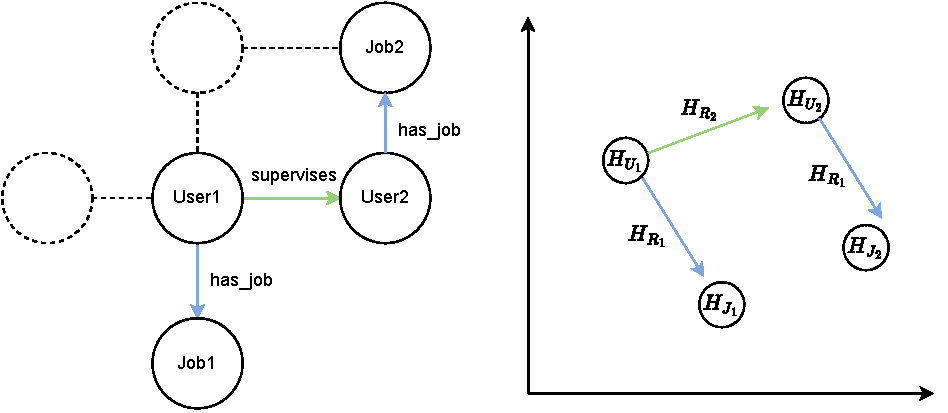
\includegraphics[width=0.8\textwidth]{img/kge.drawio (3).pdf}
    \caption[Learning node embeddings with TransE]{ Methods such as TransE map graphs into a metric space by learning node  and relationship embeddings.}
    \label{fig:kge}
   
\end{figure}
\begin{equation}
d(s,r,t) = - \| h_s + h_r -h_t \|_p
\label{eq:kge}
\end{equation}

TransE learns embeddings with the scoring function \eqref{eq:kge} such that given the edge $e, \, \psi(e)=(s,t), \, \phi(e)=r$, the embedding of node $s$, $h_s$ translated in space by the relationship-specific embedding $h_r$ is close to the embedding of node $t$, $h_t$., where  $\|... \|_p$ is the Minkowski distance. Embeddings can be learned from a random initialized lookup table and gradient descent, which the methods in the previous section use as well. Learning the relationship embeddings $h_r$ allows to apply reasoning in the embedding space. \textcite{ren2020query2box} illustrate this ability by the example of finding "Canadians which won the Turing-Award" by applying the corresponding relations "citizen" and "won" to the Canada and Turing-Award nodes to find nodes of citizens in the vicinity. The present work does not explore this dimension any further, but incorporates TransE to learn node embeddings. The example in Figure \ref{fig:kge} illustrates the need for methods like TransE, as without the relationship embeddings $h_r$ it becomes difficult to represent multiple relationship types and non-symmetric relationships in the same embedding space.  In theory, TransE can not model symmetric relationships well \parencite{sun2019rotate}, as only $h_r=\mathbf{0}$ could model such a relationship . The relationship of coworkers represents a symmetric relationship. However, TransE has been shown to still perform well despite its incomplexity when compared to more advanced methods \parencite{sun2019rotate}.



\section{Graph Neural Networks}
This section provides a brief overview over a selection of Graph Neural Network  architectures and illustrates how the training can be approached. 

Fundamentally, Graph Neural Networks are similar to the graph-based embedding methods introduced in the previous section, in that they can be utilized to compute node embeddings.  But they can be extended to edge- and graph-level tasks as well, incorporating node and edge features  and further considering different node and edge types such as present in heterogeneous graphs. Additionally, sampling methods have been developed \parencite{ying2018graph}, which allow the training of those networks on graphs with several billions of edges  using stochastic gradient descent. 
The present paper applies the Heterogeneous Graph Transformer (HGT) \parencite{hu2020heterogeneous} to a learning recommendation problem. 
The HGT builds up on several advancements in the field, introduced in the following paragraphs.


\begin{equation}
h_t^l = \sigma\left(   \sum_{s \in \mathcal{N}(t)} \frac{\mathbf{W}^l \cdot h_s^{l-1}}{|\mathcal{N}(t)|} \right) \label{eq:matrix_mult2}
\end{equation}

The concept of Graph Convolution is introduced by \textcite{kipf2016semi} with the \textbf{Graph Convolutional Neural Network} (GCN). Their initial formulation of the network considers the whole graph. This paper uses the node level formulation \eqref{eq:matrix_mult2} by the authors as the formulation is further extended upon.


The formula describes one layer $l$ of the GCN, specifically the computation of the node representation $h_t^l$ of node $t$ at layer $l$. The fundamental assumption is that nodes can be described in terms of their neighbors as well as  the “messages” exchanged with those neighbors. These interactions are modeled in two steps \eqref{eq:matrix_mult2}:

\begin{itemize}
\item Firstly, node information of the neighboring nodes is passed as message to the target node by transforming the representation $h_s^{l-1}$ of each neighbor $s$ in the last layer by the learnable matrix $\mathbf{W}^l$. 
\item Secondly, the messages of all neighbors are aggregated using a permutation-invariant transformation, such as the average, and passed through a  non-linearity $\sigma$ to create the target node's embedding $h_t^l$ at layer $l$. It has to be noted that the neighbors of node $s$ may include $s$ itself through a self-edge. Therefore, the representation $h_t^l$  of the node can consider information of its own representation $h_t^{l-1}$ at the previous layer ${l-1}$.
\end{itemize}
 

The \textbf{Relational GCN} (RGCN) \parencite{schlichtkrull2018modeling} extends the GCN to learning on heterogeneous data. Specifically, it allows to learn more accurate node representations on the heterogeneous graphs, which have different entity and relationship types. In detail, in  Equation \eqref{eq:matrix_mult2}, one distinct relationship weight $\mathbf{W}_r^l$ is learned for each relationship type $r \in \mathcal{R}$. This follows the intuition that, for example, the relationship between "authors and authors" versus "authors and papers", different dimensions of the node embeddings may be the most informative. 
 
\textcite{hamilton2017inductive} introduce the \textbf{GraphSAGE} architecture, which proposes other permutation-invariant aggregation functions such as mean-pooling, or max-pooling for GNNs. A permutation-invariant aggregation is necessary because there is no natural way of determining the order of neighbors relative to the target node. Contrary, a natural order is given in other data types such as words in a text, speech sequences or pixels in images. Using the Graph Convolution, multiple layers can be chained, where each layer takes as input the node representations calculated in the previous steps. Initial node representations can be inherent node features or artificially constructed by computing graph-structural features such as the node degree, clustering coefficient or triangle count around the node \parencite{hamilton2017inductive}. 

\begin{figure}
    \centering
    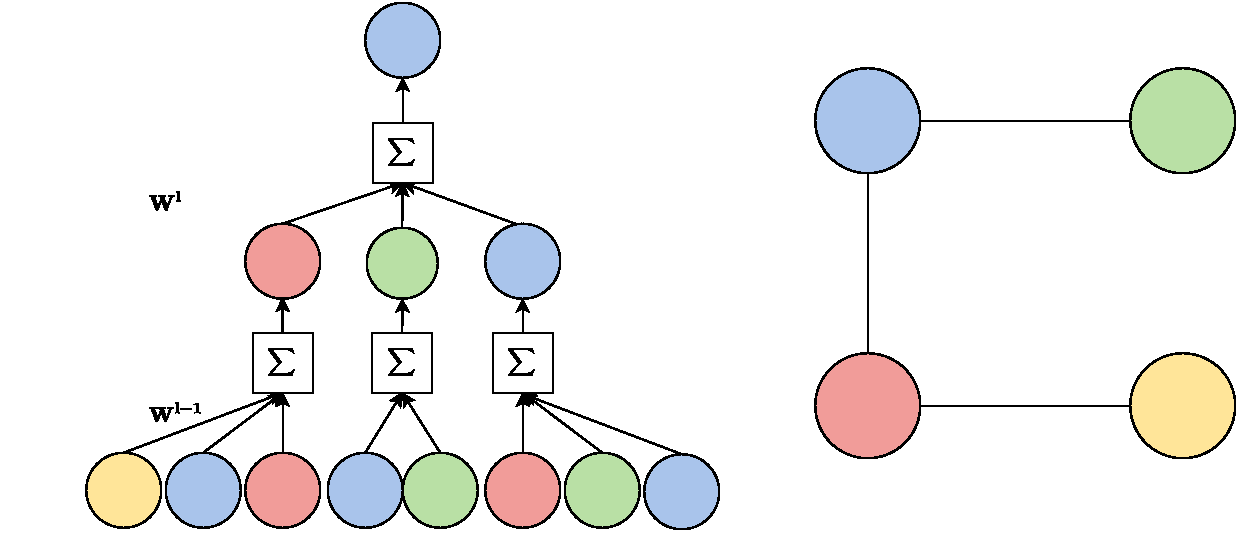
\includegraphics[width=0.8\textwidth]{img/nodecomputationgraph.drawio (5).pdf}
    \caption[Computational graph for computing a node representation]{Exemplary two-layer computational graph for computing the node representation of the blue node in a Graph Neural Network, including self loops.}
    \label{fig:compgraph}
\end{figure}

The GCN formulates the aggregation on a global level, whereby in each step, all node representations are computed taking into account all representations of their neighboring nodes from the previous step. \textcite{hamilton2017inductive} built upon the node-centric view shown in Equation \eqref{eq:matrix_mult2} in practice,  where each node creates its own computational graph (Figure \ref{fig:compgraph}). This allows training the GraphSAGE model using stochastic gradient descent with sampled mini-batches of target nodes and the nodes contained in the target nodes' computational graph. The apporach drastically reduces computational cost and enables training on large scale graphs. Further, they select neighbors randomly to reduce computational cost and empirically find for their usecase a neighborhood size of 25 one-hop and $25\cdot10$ two-hop neighbors to exhibit good performance considering the computational cost. In the present work the notion of node-centric training is utilized and the empirical neighborhood sizes are taken as reference.

Besides computational considerations, the selection of a subset of neighbors is also required for the following reason. By the way the GCN is formulated, for each added layer of the GCN, the receptive field size grows approximately by the power of the average degree. For a large layer count, the target nodes representation is computed by taking into consideration a large amount of other nodes in the graph. For the aggregation architectures introduced until now, the phenomenon known as “over-smoothing” problem \parencite{rusch2023survey} is augmented by increasing the layer count of the GNN. With increasing depth the networks is unable to compute distinguishable node representations for different nodes anymore. The Graph Attention Network aims to reduce this phenomenon.



\begin{equation}
\begin{aligned}
\tilde{\alpha}_{st} &= \mathbf{a}^T [\mathbf{W}h_{s}, \mathbf{W}h_{t}] \\
\alpha_{st} &= \frac{\exp\left(\sigma(\tilde{\alpha}_{st})\right)}{\sum_{u \in \mathcal{N}(t)} \exp\left(\sigma(\tilde{\alpha}_{ut})\right)} \\
h_t' &= \sigma\left(\sum_{s\in \mathcal{N}(t)} \alpha_{st}\mathbf{W}h_{s}\right)
\label{eq:gat}
\end{aligned}
\end{equation}




The \textbf{Graph Attention Network} (GAT) \parencite{velivckovic2017graph} introduces the attention mechanism \parencite{bahdanau2014neural} to GNNs in order to mitigate  the over-smoothing problem. The attention mechanism \eqref{eq:gat} allows the GAT to “attend” to each neighbor $j$ differently by the single scalar $\alpha_{st}$, instead of aggregating each neighbor with equal weight. Therefore, the GAT can selectively choose neighbors it deems as important with respect to computing the target nodes next-layer representation, and diminish the signal of the other nodes, whereby the oversmoothing problem is reduced. Notably, only a single attention vector $\mathbf{a}$ is learned to reduce overfitting on small datasets. In Equation \eqref{eq:gat}, the use of "$[]$" denotes concatenation.  To stabilize the learning process they further concatenate multiple attention heads to learn the final representation ${h_t}$.












 
\chapter{Related Work}
\label{ch:relatedwork}
Following works bear similar characteristics to the present work, which is the problem of recommending learning content to users as well as the graph-based approach taken.

\textcite{tarus2017hybrid} propose a hybrid recommender system which includes CF, a KG, as well as sequential pattern mining. The cold-start problem is addressed by utilizing knowledge about the learners through the KG. The authors can include detailed personal data such as learning style and knowledge level into the KG, different to the present work. They further construct two separate graphs, one for the learner and one for the learning resources. Instead of Graph Neural Networks, a hand-crafted approach is taken to compute the similarity between two learning objects.

\textcite{wang2021personalized} establish two different learning frameworks. The second is most similar to the present work. To address the sparsity problem of the skill profiles of people, they construct two graphs. The first graph connects learners which have completed the same learning content, which allows to infer their skill profile through other learners. The second graph connects the learners to peers in their department. The hypothesis is that people in the same department might share similar competencies. They then combine the knowledge from both graphs using a self-modeled GNN similar to the GAT \parencite{velivckovic2017graph}. They extract competency topics from the skill profiles of learners using a variatonal autoencoder \parencite{kingma2013auto} and model the topic demand through historical records and changes in the topic proportions. Finally, they employ CF to generate recommendations. 

Opposed to the two-graph approach in  \parencite{wang2021personalized}, the present work constructs a unified KG. Additionally to the entities and relationships in \parencite{wang2021personalized}, the present graph includes the learning content as well as the supervisors. The unified graph holds no direct skill-profiles of learners. Instead the skills are only connected to the learning content. The HGT is employed to deal with the resulting more complex relationships of entities in the graph. This unified approach of including all entities in the same graph reduces the complexity for maintenance and allows for more flexible experimentation.



\newpage

\begin{equation}
\begin{aligned}
\tilde{\alpha}(s, e, t) &= \left(K(s) \, \mathbf{W}^\text{ATT}_{\phi(e)} \, Q(t)^T\right) \cdot (...)  \\
K(s) &= \mathbf{W}^{K}_{\tau(s)}h^{l-1}_s \\
Q(t) &= \mathbf{W}^{Q}_{\tau(t)}h^{l-1}_t
\label{eq:hgt}
\end{aligned}
\end{equation}

The \textbf{Heterogeneous Graph Transformer} (HGT) introduced by \textcite{hu2020heterogeneous} builds upon the previous mentioned ideas for representation learning on heterogeneous graphs. 
The essential difference to GAT is the use of three interaction matrices  $\mathbf{W}^{K}_{\tau(s)}, \, \mathbf{W}^\text{ATT}_{\phi(e)}$ and $ \, \mathbf{W}^{Q}_{\tau(t)}$  to model each component of  the meta relation $\langle \tau(s), \phi(e), \tau(t) \rangle$ \eqref{eq:hgt}. 

%\frac{\mu_{\langle \tau(s), \phi(e), \tau(t) \rangle}}{\sqrt{d}}

They argue that the way the GAT models the attention component $\tilde{\alpha}_{st}$ with the same matrix $\mathbf{W}$ for $h_s$ and $h_t$ in formula \eqref{eq:gat} is insufficient for heterogeneous graphs as both node types might posses different feature distributions. Instead, two matrices $\mathbf{W}^{K}$ and $\mathbf{W}^{Q}$ are learned. These matrices are learned per node type  $a \in \mathcal{A}$, which allows the reuse of those weights across different edge types $r \in \mathcal{R}$, potentially towards other node types. For edge types for which data is rare and  $\mathbf{W}^\text{ATT}_{\phi(e)}$ can not be learned well, an increase in performance can be achieved by this method. As the present work deals with a heterogeneous graph where some edge types are more rare than others, the HGT is chosen. 



Additionally to the HGT,  \textcite{hu2020heterogeneous} propose a novel sampling method to sample the computational graph for target nodes contained in a single mini-batch. The method samples in a way such that for each node type an equal amount of nodes is present in the mini-batch. The probability of a node $s$ to be sampled depends on cummulated scores across the edge types  it is connected by to any target node $t$. 

One sampling iteration for a set of target nodes and the source nodes to be sampled is examined in the following. For one node type $a_1 \in \mathcal{A}$ and one edge type $r_1 \in \mathcal{R}$, for node $s$, $\tau(s) = a_1$ the score to be sampled with respect to target node $t$, $\tau(t)=a_x$, is equal to $\frac{|E_s|}{|\mathcal{N}_{r_1}(t)|}$\, where $E_s = \{e | \psi(e) = (s,t) \land \phi(e) = r_1 \}$. Intuitively, this allows to keep the sampled sub-graph of the mini-batch dense, because those neighbors are more likely to be sampled, which maintain edges to multiple different target nodes. Information loss can be reduced, because the sampled edges are more representative of the local neighborhood around the target nodes in the mini-batch, useful for sampling on large scale graphs.  Furthermore, the computational load is reduced, since a smaller amount of distinct node representations have to be computed. This sampling method is chosen in the present work as well.

The work learns the node embeddings  combining the HGT with \textbf{TransE} \parencite{bordes2013translating}. Details on the exact implementation are provided in the Methodology Chapter \ref{ch:methodology}. Specifically, a Knowledge Graph Embedding approach is chosen, as besides the user-item  recommendation task, further experiments are conducted to learn general node embeddings for all entity types. 


\begin{equation}
\begin{aligned}
\mathcal{L} &= \sum_{(s,r,t)\in S} \sum_{(s',r,t') \in S'} [\gamma + d(h_s + h_r, h_t) - d(h_{s'} + h_r, h_{t'})]_{+}\\
[a]_{+} &=  \begin{cases}
    a,& \text{if } a\geq 0\\
    0              & \text{otherwise}
\end{cases}
\end{aligned}
\label{eq:pairwise}
\end{equation}

The embeddings of the relationships are learned using pairwise margin loss \parencite{pytorchloss} as proposed in the original paper \parencite{bordes2013translating} \eqref{eq:pairwise}.



$\gamma$ is a scalar margin and $d$ is the Minkowski distance. $S'$ represents the set of tuples in which either the head or tail node is corrupted, such that the edge between the two nodes is not present in the actual data. For ease of implementation, the present paper only corrupts the tail node.

\chapter{Methodology}
\label{ch:methodology}
This chapter outlines how the experiments are conducted. The decisions are outlined, made during data selection, cleaning and preprocessing, the structuring and description of the graph as well as the architecture of the recommender system and the baselines. The reasoning is presented, how the training and test datasets are constructed, and how sampling and evaluation are carried out to ensure a fair comparison. In particular, the recommendation task is to predict the learning content a user has already completed, since this task should allow the system to learn which kind of content the user is interested in.

\section{Graph Construction}
In the following it is described how the heterogeneous graph is constructed, which includes nodes for skills, jobs, employees, their supervisors, organizations, learning content, and their relationship edges.

Data cleaning and pre-processing can be divided into three stages. 
The first stage  and the beginning of the second stage are not part of the author's work. Nevertheless they provide context, which is why they are described in the following. 

Firstly, the skill graph and corresponding skill relationships are established. Examples of skills include “programming”, “python programming” or “communication competency”, where an edge might exist between “programming” and “python programming” since they are closely related. A skill list of 260,000 skills is accumulated by combining skill lists from different sources, including the lists from O*NET \parencite{onetonline} and ESCO\parencite{escoonline}. Further skills are extracted with the help of language models from Open AI \parencite{OpenAI2023GPT4TR} from a subset of 150 million job postings including their descriptions and titles which the company has acquired. The inter-skill relationships are formed by fetching pairwise combinations of the 260,000 skills which are present in 2 million of the job descriptions. Each pair of skills is compared regarding their cosine similarity when transformed with S-BERT sentence embeddings \parencite{Reimers2019SentenceBERTSE} \parencite{sbertmodel}, and only relationships are includes for which the cosine similarity is greater than an empirical threshold.

In the second stage, skill–job relationships are formed. O*NET \parencite{onetonline} provides a list of 1000 standardized job categories. This list is expanded to each subcategory creating 55,000 individual jobs. The 150 million job descriptions are mapped to one of the 55,000 jobs using the cosine similarity of the S-BERT embeddings \parencite{Reimers2019SentenceBERTSE} between the title of the job description and the job titles of the 55,000 jobs. In the case of a low similarity to all of the 55,000 jobs, the initial O*NET category is chosen which has already been hand-annotated for each job posting. This concludes the discussion of work that falls outside of the scope of this paper. 


Relationships between jobs and skills are established with the help of the job descriptions and Term Frequency–Inverse Document Frequency (TF-IDF) \parencite{tfidf}.  Normally, TF-IDF is used to characterize documents semantically by representing them as n-dimensional real valued vector, one dimension per word in the corpus. This work reformulates this idea, where a job title corresponds to the “document”, which includes all job descriptions which have been  mapped to this job title in the previous step. The job can then be represented by an 260,000 dimensional vector, one dimension for each skill of the skills list. Each of these dimensions resembles the relationship of the job to each of the skills, which is characterized by the score of that dimension. 




\begin{equation}
\begin{aligned}
\text{TF}_{sj} &= \frac{\frac{2}{127}+\frac{5}{82}+\frac{0}{57}}{3}\\
\text{IDF}_{s} &= \ln\left(\frac{55,000}{\frac{1}{3}+\frac{1}{3}+\frac{0}{3}+x+1}\right) + 1\\
\text{TF-IDF}_{sj} &= \text{TF}_{sj} \cdot \text{IDF}_{s} \label{eq:tfidf}
\end{aligned}
\end{equation}



The following example illustrates the idea:
Given three documents belonging to the job $j$, with the relative occurrence counts of the skill $s$ in the each of the job descriptions of $j$ the $TF_{sj}$ is computed \eqref{eq:tfidf}, where each job description receives an equal weight. The inverse document frequency $IDF_s$ is then computed \eqref{eq:tfidf}, with a document frequency of $\frac{2}{3}$ of $s$ with regards to $j$ and $x$ symbolizing the document frequency with regards to the remaining jobs. The TF-IDF score then represents the importance of the skill with respect to the specific job, as it is given by the “job posting” context. By this measure, a skill $s$ is important to a job $j$ if it occurs often in job descriptions of $j$ and less often in job descriptions of other jobs. The present formulation of TF-IDF is used, which reduces the penalty on skills appearing in multiple documents compared to other formulations. Therefore, jobs are characterized by more general skills. The computation is carried out in parallel for each of the 150 million job descriptions over all 260,0000 skills with the distributed computing framework Apache Spark \parencite{zaharia2016apache}. For graph construction, all job-skill relationships with a score greater than 0 are kept. Later, for each job, only the 50 skill edges with the highest scores are used. The skill scores not only allow to rank skills by importance per job, but also enable the comparison of the importance of a skill between different jobs. Examples can be found in the Appendix \ref{ch:tfidfappendixw}.


Lastly, this skill and job graph is connected to the data collected from real customer of SAP's learning platform. The data include 300,000 employees, 60,000 courses, and 24 million completion events indicating the completion of learning content by employees. The completion of courses is a type of implicit feedback which can indicate the interest of users towards a specific type of content. Unfortunately, there is no indicator column if completion events are of mandatory nature. Naturally, these courses need to be filtered out, because they do not reflect the interests of users. For removing these courses following rules were followed. All learning events are removed, which:
\begin{itemize}
\item record completion of the same course more than once by the same person, as this may indicate periodically recurring mandatory trainings.
\item are assigned to more than three persons on the same day. This information is included in the completion records. The threshold is empirically determined and is set conservatively to rather filter out a larger number of events.
\item are assigned to more than one person by the same person, as this indicates a supervisor assigning courses to supervisees.
\end{itemize}

The success of these rules is shown with the following calculation. The percentage of events containing the strings “mandatory” or “complian” in the text of the course is compared for events which are filtered out and kept. For the 23,44 million events which are filtered out, 1.02\% contain one of the strings, whereas only 0.15\% of the 560,000 events which are kept contain the strings. As expected, most recorded events are mandatory. A small percentage of French and Spanish job titles of people as well as titles and descriptions of courses are translated with an automated online translation tool. To form the course–skill relationships which indicate if a course teaches a skill, the S-BERT \parencite{Reimers2019SentenceBERTSE} language model is  trained on tagging skill terms in the course title and description, which is not part of the author's work. The extracted skills are matched against the existing 260,0000 skill list with the Levenshtein distance \parencite{levenshtein1966binary}, which allows non-exact string matching. The remaining extracted skills are matched to the skill from the skill list with the highest cosine similarity of both S-BERT \parencite{Reimers2019SentenceBERTSE} embeddings. Extracted skills with which cannot be matched by non-exact string matching or a high cosine similarity are discarded.  In summary, the relationship between skills and courses are derived through the skills mentioned in the descriptions of courses. In a similar manner, the job titles of employees are matched with one of the 55,000 standardized job titles to obtain the job-employee edges which indicate the job of the employee.
Other relationships extracted from the data include
qualifications, which can contain multiple courses and have text
descriptions as well. Employees can be part of organizations and can have supervisors. Cleaning decisions such as handling partially duplicate, incomplete or ambiguous data are not discussed.


\begin{figure}
    \centering
    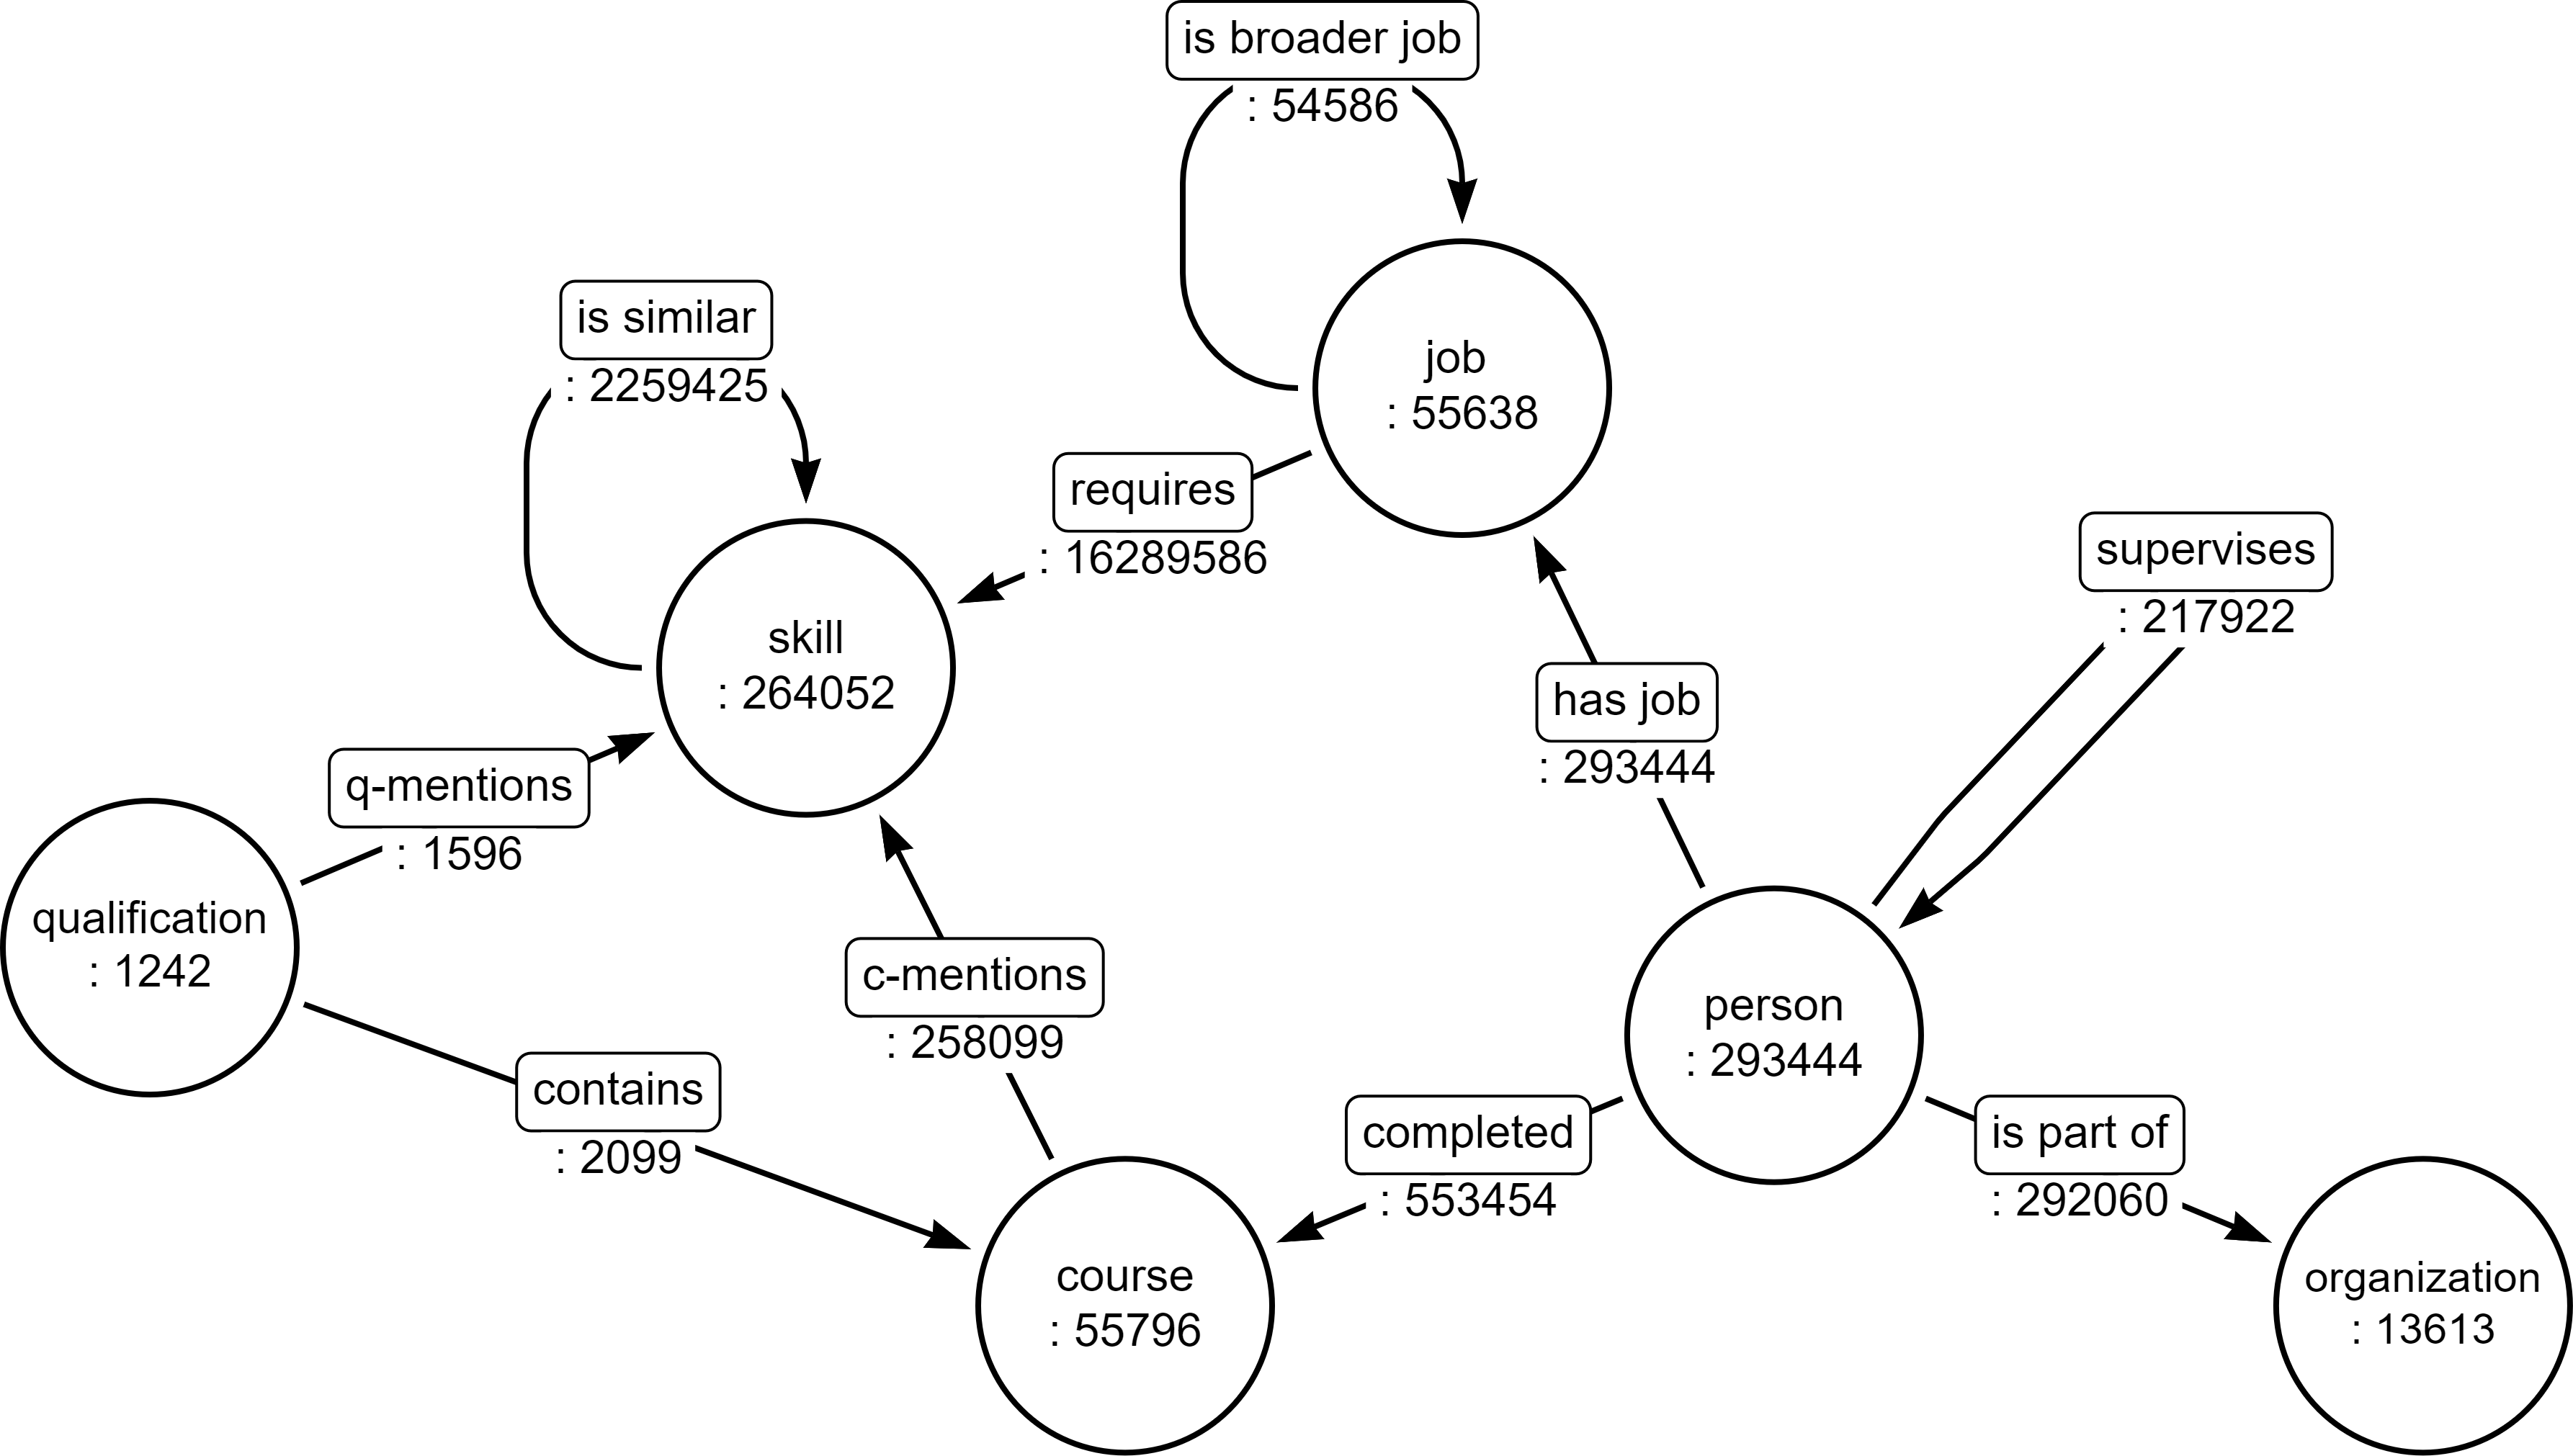
\includegraphics[width=0.8\textwidth]{img/heterogeneousgraph (6).png}
    \caption[The heterogeneous Graph]{The final heterogeneous graph with corresponding node and edge amounts}
    \label{fig:graph}
\end{figure}

 Figure \ref{fig:graph} illustrates the entity relationship diagram together with the realized numbers of entities and relationships. 
Although the figure depicts directed edges for semantic clarity, the sampling approach utilized to train the HGT and the baselines considers the undirected version of the graph, where an edge exists in both directions. It further has to be noted, that degree distributions of $\tau(s)$ and $\tau(t)$ regarding $\langle \tau(s), \phi(e), \tau(t)$ must not necessarily be similar.  Figure \ref{fig:entities2} shows the degree distributions of nodes for a subset of the edge types. Examining the degree distributions, large differences exist. Most of the 300,000 employees have not completed a learning, whereas most jobs are connected to at least 9 skills. During GNN-training the employed HGT-sampling approach helps to alleviate these differences. 

To reduce the complexity in the training process and filter out skills with low importance, the edges of jobs to skills are limited to the 50 skills with the highest TF-IDF score with respect to the job, which reduces the edge count to about 1.2 million edges. No further analysis regarding the graph structure such as computing the diameter, the longest shortest path between two nodes,  of the graph is conducted, as it is not crucial to the task at hand and it is found that specialized tooling would be needed to conduct the analysis on the large graph. 
\begin{figure}
    \centering
    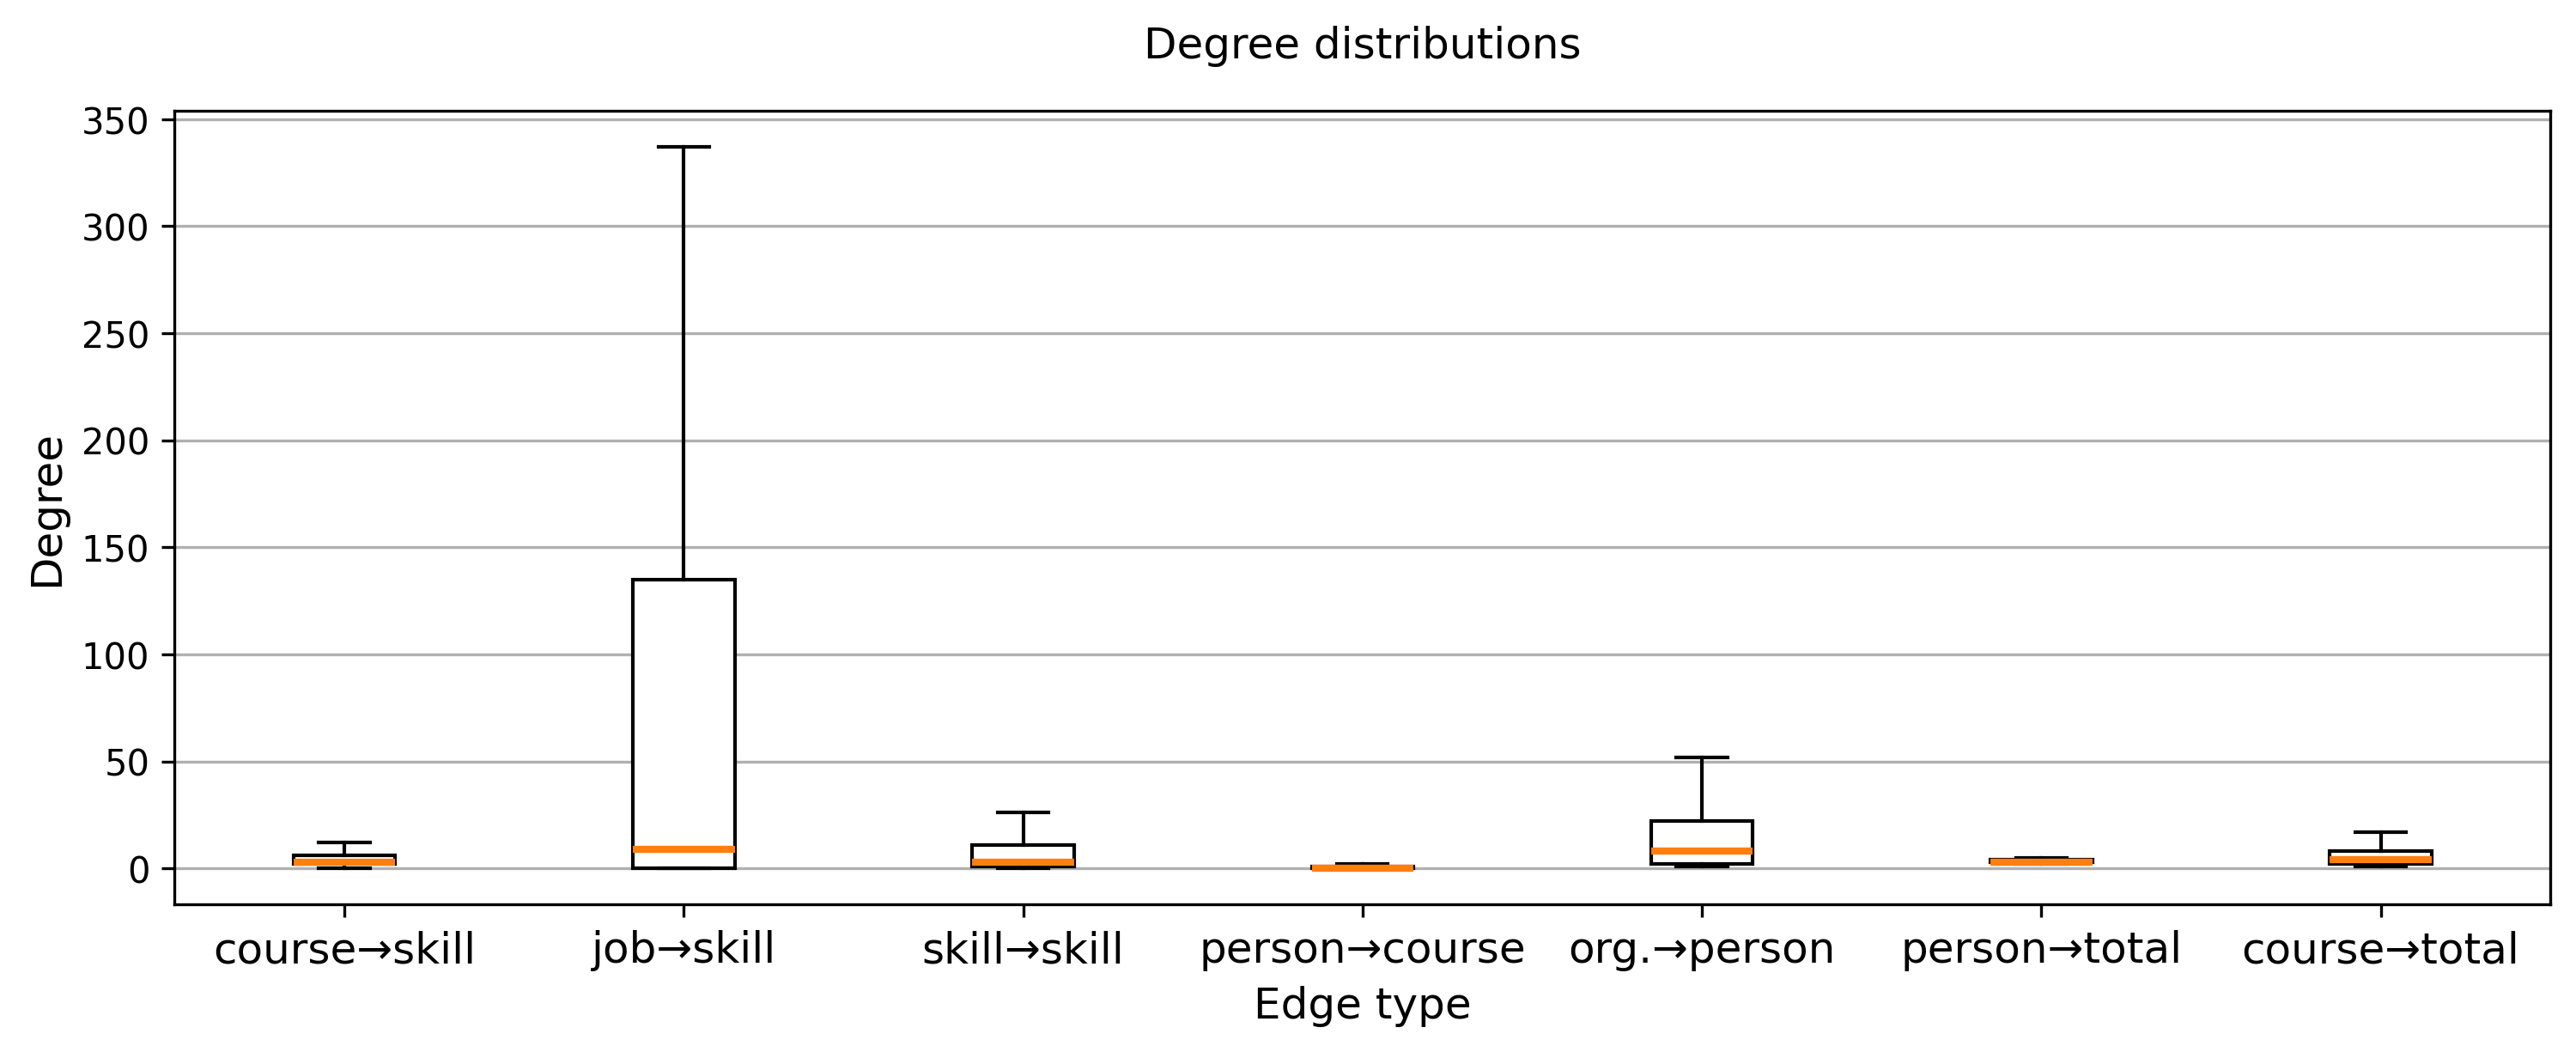
\includegraphics[width=0.8\textwidth]{img/boxplot_notable_notable.png}

    \setlength\tabcolsep{3pt}

\begin{tabular}{|c|c|c|c|c|c|c|c|}
\hline
 & course→ & job→ &skill→& person→  & org.→  & person→ & course→ \\ 
 & skill & skill & skill&course &person&total&total\\
\hline
  Q3 & 6 &135&11&1&22&4&8 \\ \hline
 Median& 3&9&3&0&8&3&4\\ \hline
 Q1 & 2&0&1&0&2&3&2\\ 


\hline 



\end{tabular}

    \caption[Node degree distributions]{A subset of degree distributions of the links of the respective first entity type to another entity type in the graph, excluding outliers}

    
    \label{fig:entities2}
\end{figure}

 \section{Structural Graph Features}
  \begin{figure}
    \centering
    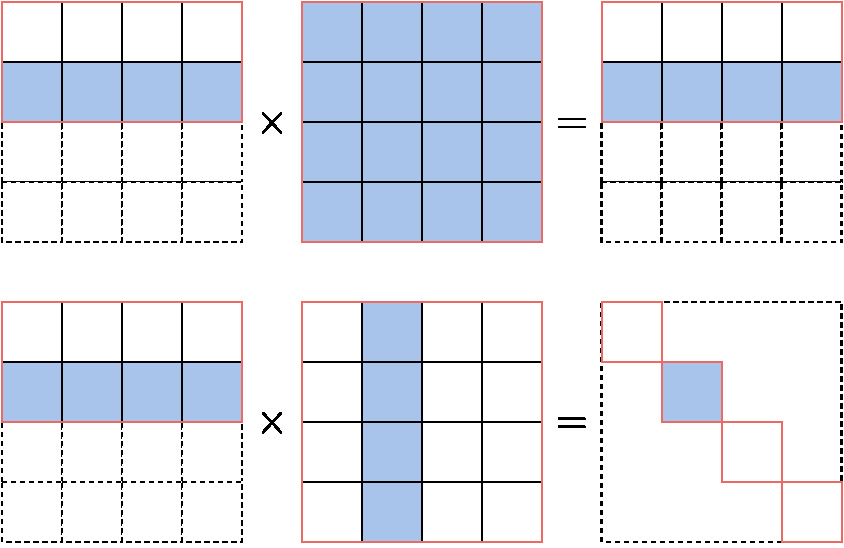
\includegraphics[width=0.8\textwidth]{img/sparsemul.drawio (1).pdf}
    \caption[Triangle count matrix calculation]{Exemplary procedure of calculating the triangle count on sparse matrix representations of the adjacency matrix in mini-batches of two nodes in two calculation steps. The red markings show the parts of the matrix present in GPU memory in each step.}
    \label{fig:computetriangle}
\end{figure}
To allow a fairer comparison, structural graph features are added to the graph's node features, since the baselines have no access to the graph structure, whereas the GNN can access the structure by neighborhood aggregation. The features are computed on the undirected graph. To each node's existing features, its degree count per edge type as well as the total degree count is added. 
 \begin{equation}
 t_{n_i} = \frac{1}{2}\cdot( A^3)_{ii} \label{eq:triangle}
 \end{equation}
 Similarly, the count of triangles, a node $n_i$  is part of, per edge type and in total, is included \eqref{eq:triangle}. The triangle count is an indicator for how dense the network is around the node. It can be computed using the adjacency matrix $A$. 
 
  \begin{equation}
\begin{aligned}
 4\cdot 10^7 &\ll 680,000^2\\
 1 &\ll 11560\\ \label{eq:smaller}
\end{aligned}
 \end{equation}
 
 Practically speaking, the adjancency matrix is too large to fit into the memory of the NVIDIA Tesla T4 GPU used. Fortunately, it is sufficiently sparse \eqref{eq:smaller}.
 
 



 Furthermore, the calculation can be executed separately for each node. Therefore, the calculation is done in mini-batches of 40 nodes to maximize the speed, using sparse matrices \parencite{pytorch_sparse} (Figure \ref{fig:computetriangle}). The mini-batch size is limited by the available memory on the GPU.  


  






 

\section{Proposed Recommender System}


  \begin{figure}
    \centering
    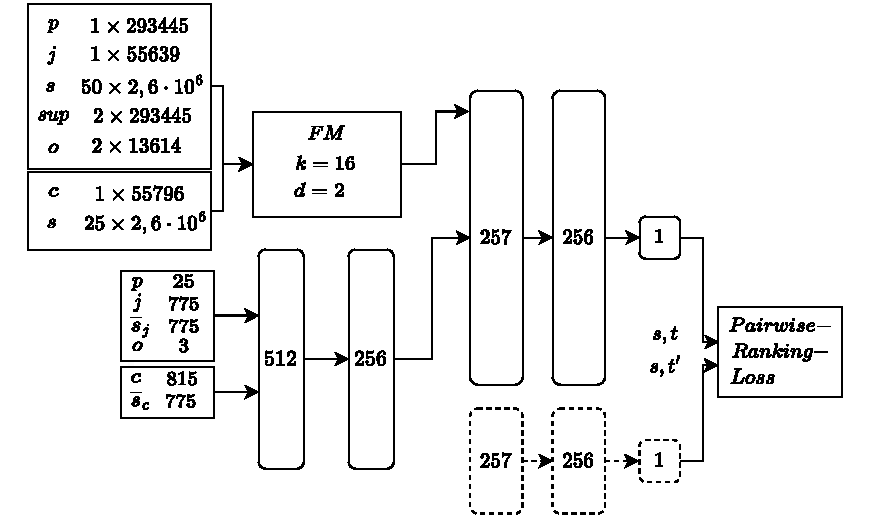
\includegraphics[width=0.8\textwidth]{img/baseline.drawio (4).pdf}
    \caption[The architecture of the second baseline]{The architecture of the second baseline model with neural network layers, the dimensions of the input data and the training setup }
    \label{fig:baseline}
\end{figure}

As  \textbf{baseline} for comparison with the proposed recommender system,
a Factorization Machine
\parencite{rendle2010factorization} is utilized. The FM can generalize on sparse data such as the dummy encoded users and items well, as mentioned in the Preliminaries. Beside user-item interactions, the FM can also include additional categorical features, such as the user's job, to mitigate the cold start problem and generalize more easily. FMs combine collaborative filtering and content based filtering, as the weight vectors $v$ can be learned through the interactions of other users regarding the items, if no explicit interactions exist for a particular user. Further, the authors show that they can mimic a number of other factorization models \parencite{rendle2010factorization}. Therefore, the FM is chosen as representative of this class of models, which has been proven to show good performance on recommendation tasks in the past such as the Netflix Prize \parencite{freudenthaler2009factorization}.


According to the authors' recommendation \parencite{rendle2010factorization}, the matrix $\mathbf{V} \in \mathbb{R}^{n \times k}$ is learned with a small dimension of $k=16$ to allow better generalization between features. Also only two-way interactions are modeled, $d=2$. The implementation used \parencite{torchfm} can not integrate continuous numerical features, but only dummy encoded categorical ones. Consequently, a second baseline is employed, which combines the FM together with a feed forward neural network layers \parencite{rosenblatt1958perceptron} to include the continuous numerical features of employees, courses and further entities. Figure \ref{fig:baseline} depicts the architecture of the second baseline, including the input feature dimensions of the data used for training. The first baseline only consists of the FM. Different architectures for the neural network layers are explored such as transforming the peoples' and courses' continuous features to the neural network separately in the first two layers. The configuration depicted in the figure achieved the best results.  

Input features to the FM are the person's and the course's categorical features.  The person's categorical features include the person, their job, the 50 skills with the highest TF-IDF score regarding the job, the person's supervisor(s) and organization(s). The course's categorical features include the course and 25 skills with the highest TF-IDF score regarding the course. Input to the neural network are the same features the proposed GNN-based system has access to. This includes 768-dimensional sentence embeddings \parencite{song2020mpnet} \parencite{sbertmodel2} of the job title of the person. The average of the skills' embeddings which are connected to the person's job title are included as well. Similar features for the course and it's skills are added. For courses, also the average user-rating and the number of ratings is given.  Further, the structural graph features discussed in the last section are provided. It is chosen not to include the qualifications in the training data. As categorical features, the qualifications would provide diminishing benefit, as no qualification is connected to more than two courses. Further, their text descriptions were found to be mostly those of the underlying courses, providing no benefit as input to the neural network either. 

The \textbf{proposed system} consists of an initial feed forward layer per node type followed by multiple HGT layers with eight attention heads each\parencite{hu2020heterogeneous} \parencite{pyg} computing 256-dimensional intermediate node representations. Three different variations are trained with two, three, and four HGT layers, respectively. 

 \begin{figure}
    \centering
    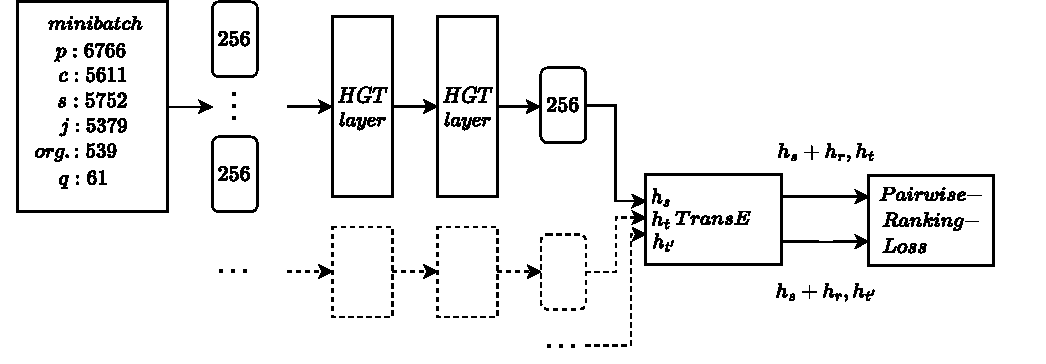
\includegraphics[width=0.8\textwidth]{img/proposed.drawio (3).pdf}
    \caption[The architecture of the proposed recommender system]{The architecture of the proposed two-layer recommender system and training approach is depicted. The left shows the example node counts contained in a sampled subgraph of neighbor-depth 4, with 32 target edges.}
    \label{fig:proposed}
\end{figure}

The final node embedding is computed by a feed forward layer before it is passed to the TransE \parencite{bordes2013translating} head. The TransE head is employed to learn the embeddings for the meta relation (user, completed, course). 

Importantly, the same loss function as in the baselines, pairwise margin loss is utilized with the same margin $\gamma=0.5$ and Minkowski distance with $p=2$ for comparability. The HGT \parencite{hu2020heterogeneous} is chosen to represent the GNN approach to recommender systems, because of the added expressivity for computing node embeddings on heterogenous graphs of the HGT, compared to the GAT \parencite{velivckovic2017graph} and the RGCN \parencite{schlichtkrull2018modeling}. It further shares entity weights across relationship types, which is beneficial for the present graph, as some meta relations with a small number of realizations such as (qualification, q-mentions, skill) exist. For this meta relation the attention weights learned with (skill, is-similar, skill) and (course, c-mentions, skill) can be reused for better performance. The whole system is depicted in Figure \ref{fig:proposed}.

\section{Training}
 \begin{figure}
    \centering
    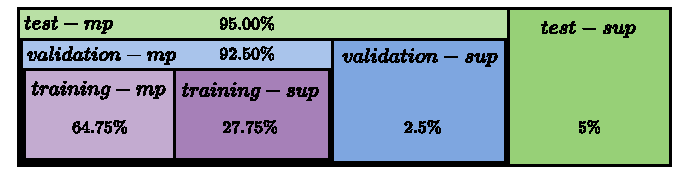
\includegraphics[width=0.8\textwidth]{img/datasetsplit.drawio (1).pdf}
    \caption[Edge-level graph split]{The graph is split on the edge level. The message passing and supervision edges of the previous split constitute the message passing edges of the next split. }
    \label{fig:split}
\end{figure}


The problem of learning recommendation can conceptually be defined as link prediction for the baselines as well as for the GNN-based system. During training, the systems have to predict if a given user has completed a learning. By predicting this implicit user feedback, the systems can learn user preferences and as a result recommend more relevant courses.  The pairwise margin loss penalizes the systems when non-existent completion events rank higher than the real event or their score comes within vicinity of the score of the existing event by the margin $\gamma$. The graph is split on edge basis into train, validation and test splits, as implemented in the library Pytorch-Geometric \parencite{pyg}. For the GNN, it is chosen to separate edges used for supervision from those used for message passing (Figure \ref{fig:split}) for a more robust evaluation. For all systems, only the supervision edges are used for training with regards to the prediction task. The message passing edges are used to create the input features for the baselines and for neighborhood aggregation in the GNN-based systems. 

For simplicity, the sampling is only implemented in such a way that given a user $s$, one positive $t$ and one negative $t'$ is sampled, not reversely. This also represents the task to be solved more naturally, opposed to selecting a specific learning and predicting which users have completed it. The negative $t'$ is sampled in an approximate way, potentially allowing for false negatives. 
\begin{figure}
    \centering
    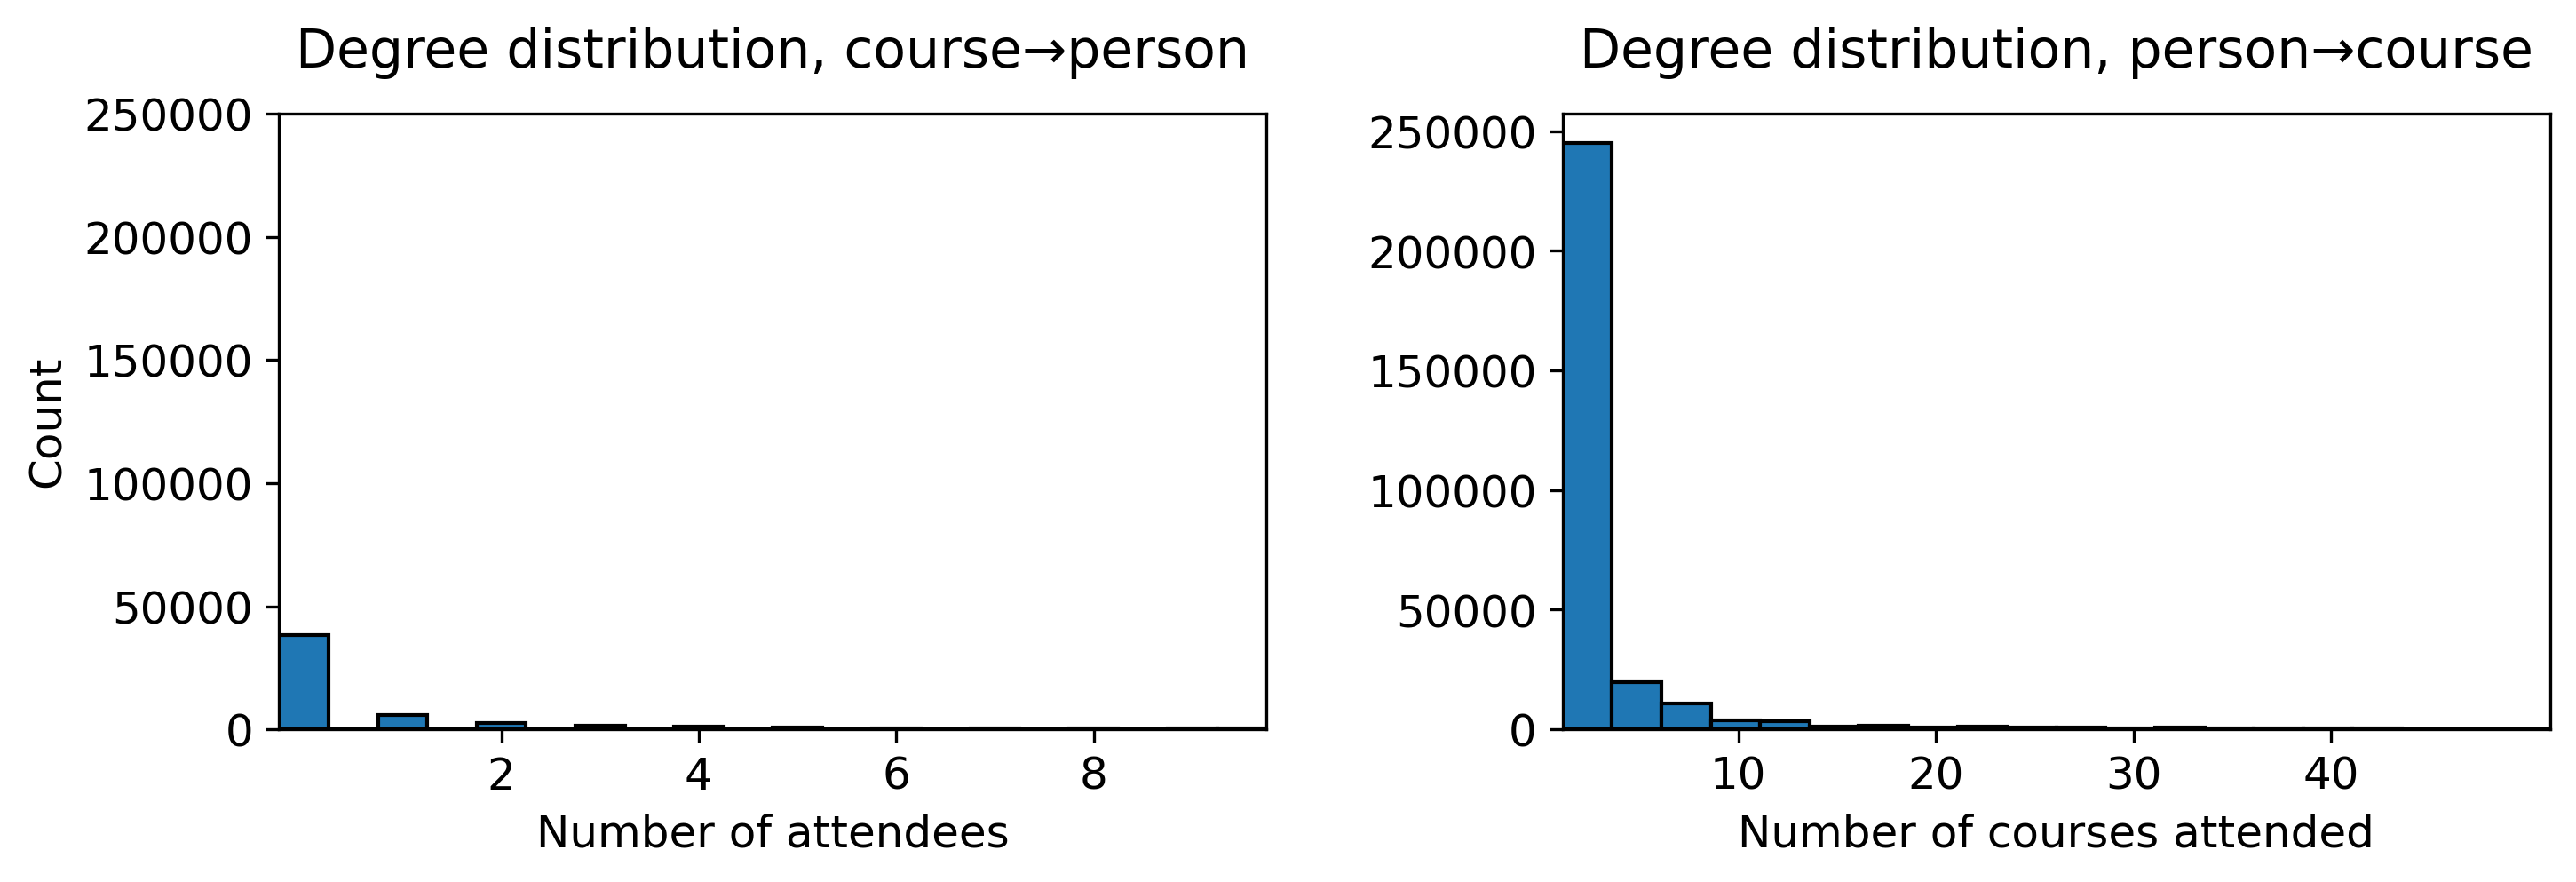
\includegraphics[width=0.8\textwidth]{img/degree_distribution_people.png0.0_14890.0_median0.0_people_min0.0_max392.0_med0.0.png}
    \caption{Degree distributions of the course-person edges}
    \label{fig:personcoursedegree}
\end{figure}
As most users have completed less than 10 courses (Figure \ref{fig:personcoursedegree}), this should not hinder performance.
The edge based split is performed for all edge types of the undirected graph, since the edges are used for a further experiment where all relationships are predicted. The aim of this additional experiment is to investigate the general quality of the node embeddings, when trained on this multi-objective problem.

Notably, by splitting the graph on an edge level, the systems can already have seen the people and courses  present in the edges of the test set, although they will not have seen the testing edges themselves. All systems are optimized with stochastic gradient descent \parencite{robbins1951stochastic} with mini-batch size of 32 and the Adam optimizer \parencite{kingma2014adam}. For each system, the best learning rate out of $\{2\cdot10^{-4}, 2\cdot10^{-5}, 2\cdot10^{-6}\}$ is selected as $2\cdot10^{-4}$. No further hyperparameter optimization is conducted to allow for a fairer comparison. 

\section{Subgraph Sampling}
The HGT-sampling is implemented in the following way:

First, a mini-batch of 32 person-course supervision edges is sampled. For each person node, a random edge to any course node is constructed. Then, the sampling approach used to train the HGT originally \parencite{hu2020heterogeneous} constructs two subgraphs for the target person nodes and the target course nodes separately. Lastly, the HGT computes node embeddings on these subgraphs to create node representations for the persons and courses respectively, and the pairwise margin loss is computed with the sampled supervision edges.

As explained previously, the specific sampling approach allows to keep the sub graph dense, meaning the supervision edges have a larger neighborhood overlap.  By selecting neighbors nodes which are shared, the sampling approach can reduce the amount of noise in the mini-batch.  It further helps to decrease the memory consumption and the computing time. Since the HGT itself will  distinguish between more informative neighbors through the attention mechanism, with larger computational resources, the HGT sampling could perhaps be omitted. 

The counts of the sampled nodes of a subgraph for the four-layer HGT are depicted in Figure \ref{fig:proposed}. The sampling approach is able to keep an equal amount of nodes per node type, approximately 5000 to 6000, for which there are enough neighbors at each sampling depth. The sampling is carried out in such a way that for the 32-node mini-batch, the neighbor limits for each node type at each depth are set to 133, 1333, 1333 and 1333 respectively. This roughly corresponds to the empirical findings of \parencite{hamilton2017inductive} of 25 one-hop and $25\cdot10$ two-hop neighbors. For the depths three and four, the amount is limited by computational resources.  
Because of the sampling method used, it is however likely that target nodes share their neighbors, and thus have access to a larger than the average neighbor amount. 
The same sampling approach is conducted for the general link prediction, where all edge types, for simplicity only in one direction, are predicted. The target edge type for each mini-batch is sampled uniformly at random for the general link prediction case. 






\chapter{Experimental Results}
\label{ch:experimental}
\begin{figure}[h]
    \centering
    \begin{minipage}{0.9\textwidth}
        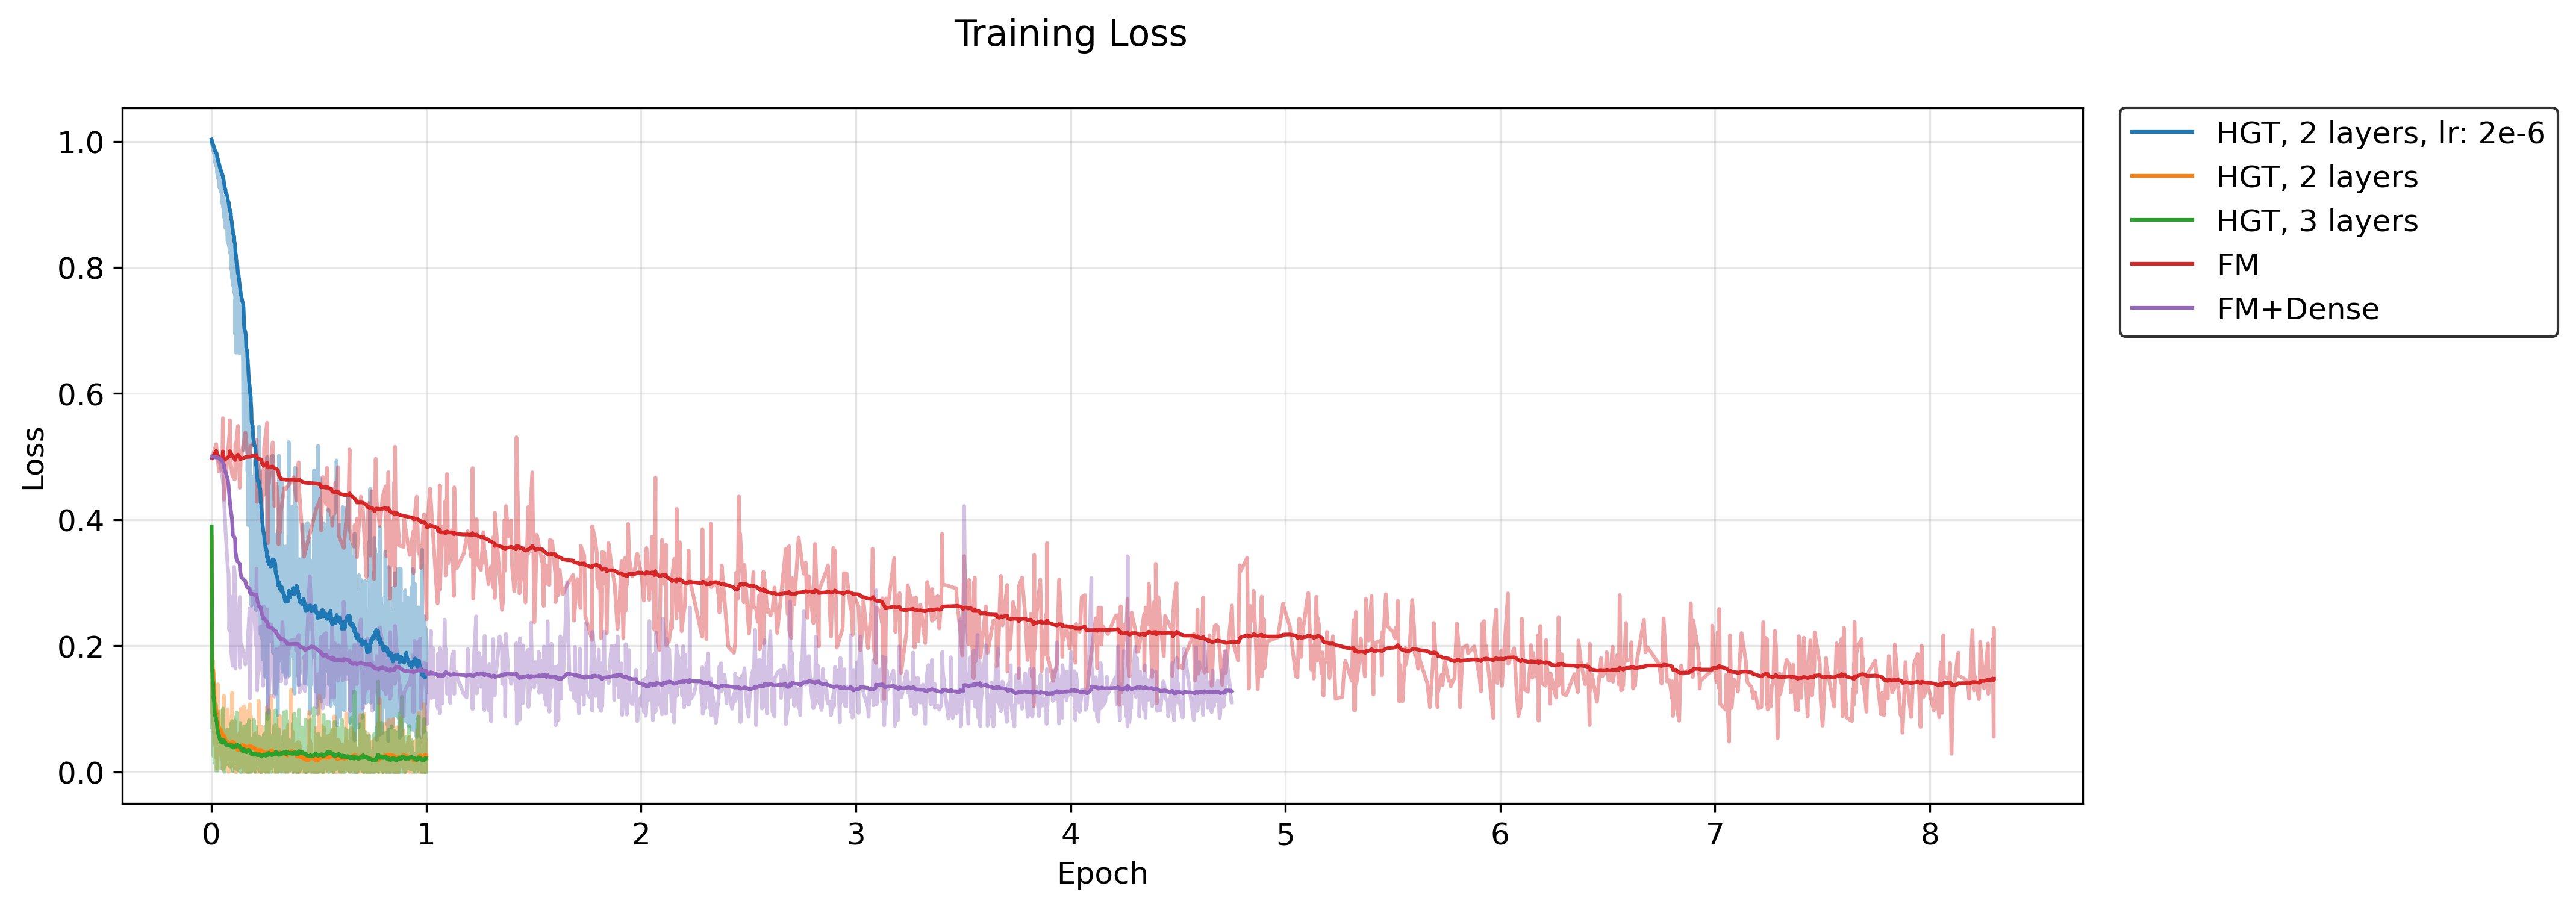
\includegraphics[width=\textwidth]{img/trainloss.png}
       
    \end{minipage}
    
    \begin{minipage}{0.9\textwidth}
        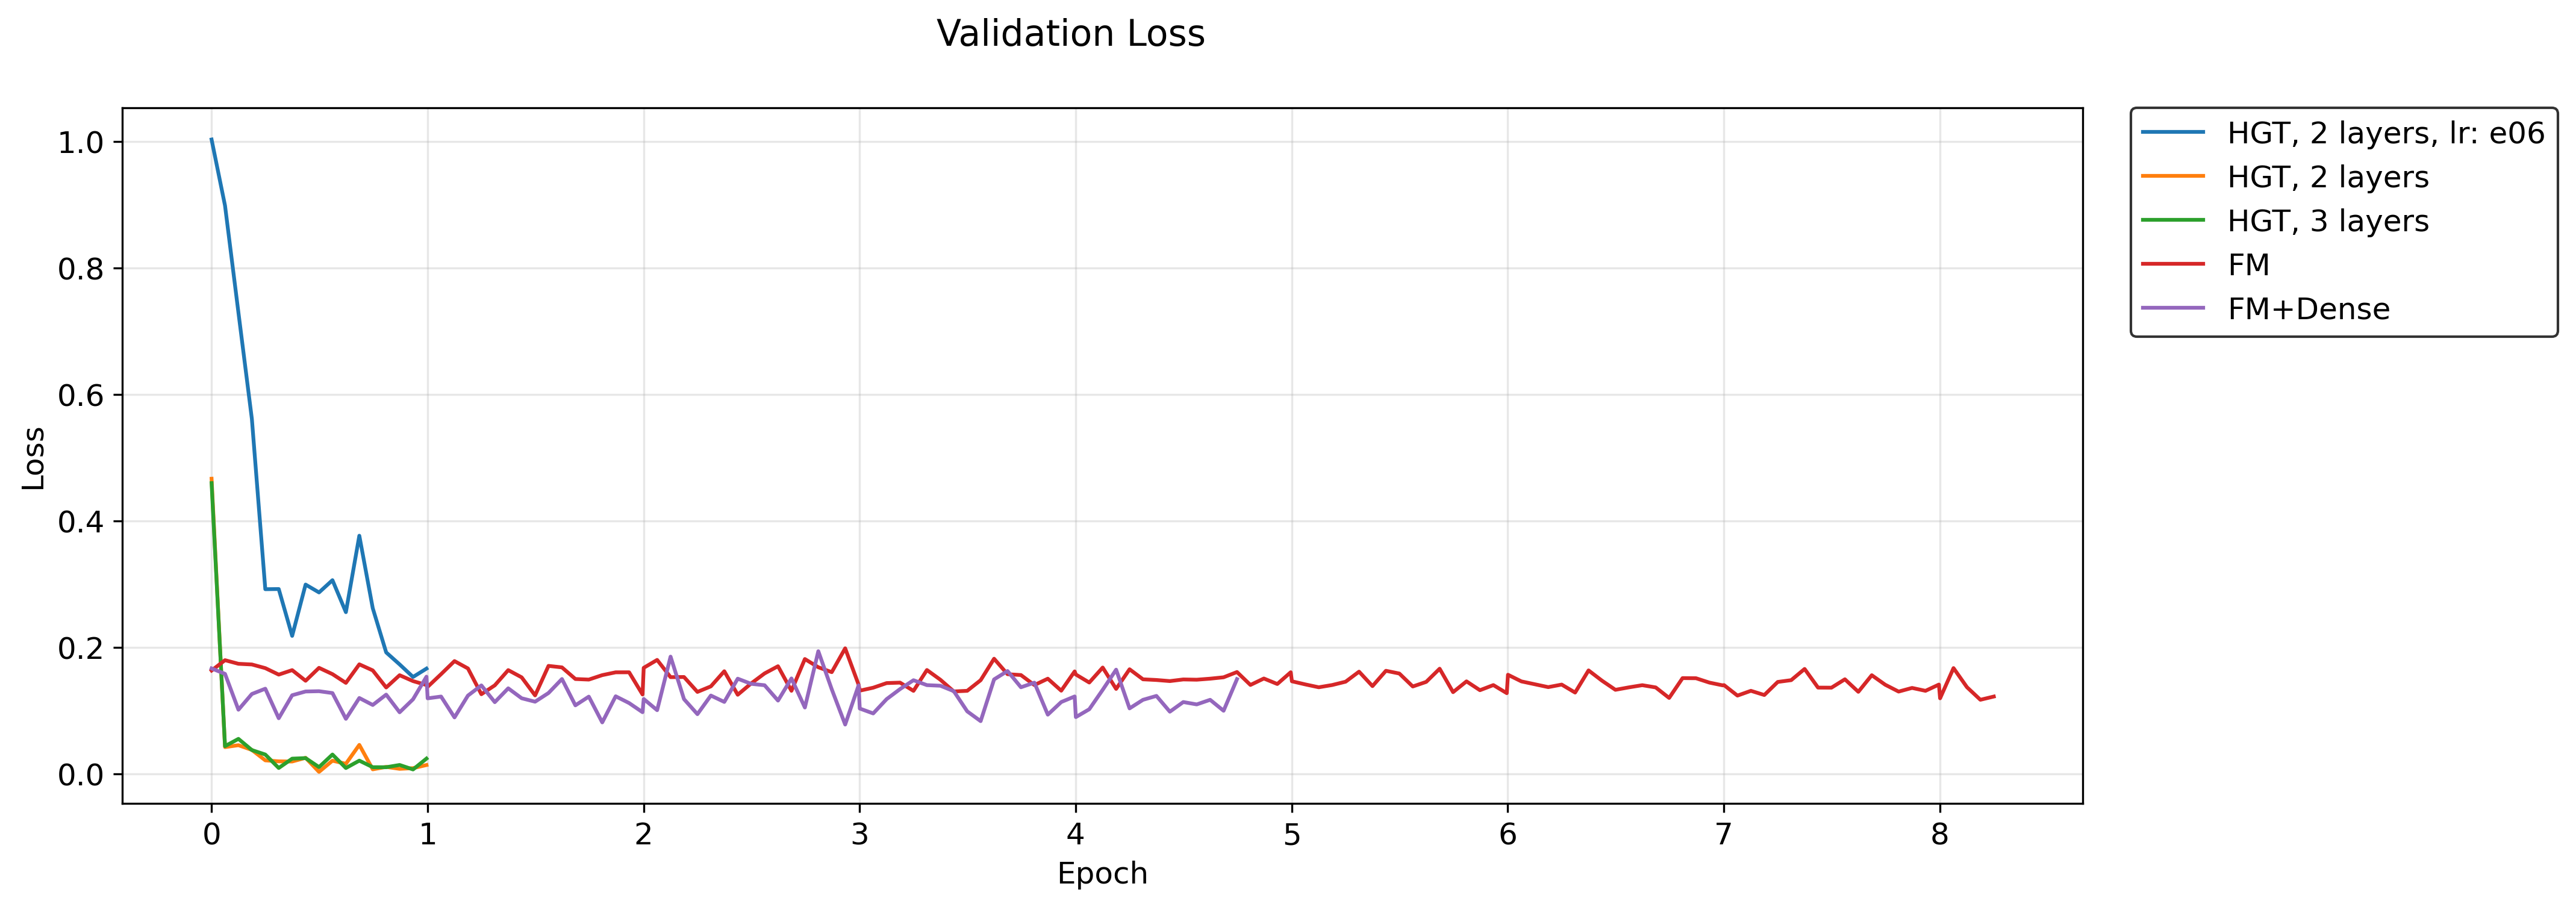
\includegraphics[width=\textwidth]{img/valloss.png}
       
    \end{minipage}
        \caption{Training and validation loss of the baselines and GNN-based systems}
     \label{fig:valloss}
\end{figure}

Each of the GNN-based systems is trained for one epoch only due to computational constraints. The duration of training one epoch on the NVIDIA Tesla T4 GPU is five hours. The baseline systems are trained for additional epochs until their loss converges on the training set, as no large loss decrease on the validation set is visible. Later, the second baseline is trained for further 59 epochs to ensure that the validation loss does not decrease visibly beyond the point depicted in Figure \ref{fig:valloss}. 

Training the baselines for more epochs is required for a fair comparison as the GNN has technically seen more data during one epoch, the node features of the whole subgraph, whereas the baselines only see the categorical, handcrafted and averaged features. The training loss on the mini-batches is smoothed for better comparability, and the real values are provided in faded colors. Validation loss is not computed on the whole validation set but mini-batches only, for performance reasons. The models' complexity is not comparable by parameter count, as the FM will only use a small subset of parameters for the categorical features during computation and the GNN-based systems active parameter count is dependent on the sampled subgraph. For reference, the second baseline has $350\cdot10^6$ trainable parameters, the three-layer HGT $\,5\cdot10^6$ trainable parameters.

The HGT with the worst performance, the learning rate of $2\cdot10^{-6}$ is included as reference as the validation loss is comparable to the loss of the baselines, and could surpass their loss as indicated by the curve of the training loss. The four-layer HGT performs similar to the other depicted HGTs, hence it is not included in the evaluation. The baseline which includes the continuous numerical features has in tendency slightly lower validation loss than the FM. The final validation losses on the mini-batches are 0.166, 0.150, 0.122, 0.024 and 0.014 respectively.




\begin{table}
\centering

\begin{tabular}{|c|c|c|c|c|c|}
\hline
Split: & \multicolumn{2}{c|}{Train} & \multicolumn{2}{c|}{Test} \\
 \hline
  & MRR & Mean Rank & MRR & Mean Rank \\
\hline
FM &  0.024 $\pm$0.073 & 5374 $\pm$ 11418& 0.014 $\pm$ 0.104 & 7749 $\pm$ 12796 \\
\hline
FM+NN & 0.075  $\pm$  0.183&2799 $\pm$ 6843& 0.074 $\pm$ 0.179 & 2981 $\pm$ 7207 \\
\hline
HGT, 2 layers & 0.380 $\pm$ 0.440 &  1122 $\pm$ 5193 & 0.368 $\pm$ 0.449 & \textbf{880.5} $\pm$ 3741 \\
\hline
HGT, 3 layers &  0.484 $\pm$ 0.478 & 1956 $\pm$ 5052 & \textbf{0.524} $\pm$ 0.487  &  1776 $\pm$ 4179  \\  \hline
\end{tabular}
\caption{Final MRR and mean rank}
\label{tab:finalscores}

\end{table}


Table \ref{tab:finalscores} depicts the MRR and mean rank obtained on all target edges from the train and test set. The rank of the positive edge is tested against all 55,000 negative edges to other courses. The three-layer HGT outperforms the best factorization based solution by 0.450 in MRR on the test set. Still, the three-layer HGTs' test MRR has a large sample standard deviation of 0.487. The addition of the continuous numerical features to the baseline improves test-MRR by 0.06. Interestingly, the two-layer HGT has a better mean rank than the three-layer HGT. The results are further discussed in the next chapter. Surprisingly, the MRR of the three-layer HGT and the mean ranks of both HGTs on the test set are better than on the training set. This is attributed to the larger training supervision-set size of 27.75\% compared to the test set size of 5\%.  


\begin{table}[h]
\centering

\begin{tabular}{|c|c|c|}
\hline
Edge Type & Train & Test \\
 \hline
  & MRR & MRR\\
  \hline
Mean &  0.090 & 0.080   \\
\hline
skill→job & 0.128 & 0.094  \\
\hline
skill→qualification &0.067 & 0.077  \\
\hline
skill→skill & 0.126 &0.064 \\
\hline
job→job &0.122 & 0.131\\
\hline
job→person & 0.065 &0.074 \\
\hline
skill→course & 0.059 &0.062 \\
\hline
course→person & 0.108 &0.063 \\
\hline
course→qualification & 0.105 &0.074 \\
\hline
job→broader job & 0.046 &0.083 \\
\hline
person→organization & 0.103 &0.088  \\
\hline
person→supervisor & 0.053 &0.066 \\
\hline

\end{tabular}
\caption[General link prediction scores]{General link prediction scores, computed on a subset only}
\label{tab:finalscoresgeneral}

\end{table}

Notably, for the computation of the test scores of the GNN, the same sampling implementation as during training is utilized. Perhaps even better scores can be obtained by computing node embeddings multiple times on differently sampled subgraphs and by averaging the results. A qualitative example of content recommended by the three-layer HGT is provided in the Appendix \ref{ch:recommendedcontent}.



Table \ref{tab:finalscoresgeneral} shows the results of the general link prediction. Scores are only approximate, as they are computed on only 1000 edges per split. 

\chapter{Discussion}
\label{ch:discussion}
The results in Chapter \ref{ch:experimental} show that the GNN-based systems can significantly outperform the factorization based approach. Furthermore, the baselines are unable to generalize as seen in the validation loss and test MRR. The results show that the added continuous numerical features increase the baselines' performance. The significant performance differences highlight the benefit of the GNN-based approach. Unlike in the baselines' case, where features such as the skills of a job are arbitrarily aggregated by taking their mean, the GNN, and especially the attention based HGT can choose to weigh the importance of neighbors differently, and aggregate depending on the neighborhood context. This illustrates that for this particular problem, manual feature engineering and experimentation would be required for the FM to achieve comparable performance to the GNN-based approach. Compared to tabular data, the graph can model the relationships between entities allowing the GNN to consider the most important relationships. 

It is further investigated if a deeper GNNs would increase performance, as it was hypothesized that the four hops would allow the model the access to the skills of peoples' neighbors' jobs. However, the results show that even a two-layer-deep GNN has sufficient performance. Comparing the two and three-layer HGT, the three-layer HGT has a higher MRR, but also the mean rank is lower. Therefore the three-layer model may have overfit sections of the graph, on which it generates more accurate predictions compared to other regions, whereas the two-layer model performs more consistently. The observation also aligns with other work such as \parencite{ying2018graph} and \parencite{hamilton2017inductive} which report diminishing performance-returns for increased layer counts beyond two for user-item interaction settings. In a different setting like fraud detection in financial systems, one could imagine more complex entity interactions to be descriptive and therefore the necessity for deeper networks could be given. 

Whereas relatively, the GNN-based approach outperforms the baselines, no claim towards the general quality of the GNN-based recommendations can be made. Explainability frameworks such as the one proposed by \textcite{amara2022graphframex} can help to trace the exact neighbors which contributed to the scores calculated by the GNN. This might help to uncover unwated biases which could be of ethical nature or caused by customer specific graph structures, which could also explain the large standard deviation in the test results. But in general, the large performance differences between certain edges has to be investigated in detail, as consistent performance is crucial to a recommender system. Additionally, the explainability frameworks could help supervisors in the decision-making process of assigning specific learnings or creating learning content which appeals to employees. 

Practically speaking, maintaining the data in a graph allows to formulate all other link prediction tasks as well. In the Human Resource setting, this could for example allow matching candidates to job offerings. Once the graph is created, the experimental iteration is straightforward. \textcite{you2020design} show that the best GNN designs are highly task specific. Therefore, the hyperparameter space of the recommender system architecture should be further explored to increase performance. 

By training the GNN on general link prediction it is shown that the model still exhibits considerable performance. The embeddings represent both the entity interactions between different entity types in the graph as well as feature aggregations. Since the TransE method embeds all nodes in the same embedding space, node embeddings obtained this way can easily be utilized in further downstream tasks in the Human Resource context, like matching candidates to job positions by comparing their similarity in the embedding space. 






\chapter{Conclusion}
In the present work, the performance of a GNN-based recommender system is compared against a traditional factorization based approach.  For this purpose a heterogeneous Knowledge Graph is constructed which combines the working and learning contexts of employees and learning content. It is shown that the graph based approach can outperform the factorization based system in the task of recommending learning content. The GNN is able to learn appropriate aggregation functions, without the need of manual feature engineering. The aggregation depends on the neighborhood context of nodes and enables the creation informative user and learning content embeddings. 

A two-hop deep HGT \parencite{hu2020heterogeneous}, compared to a deeper HGT, is shown to exhibit sufficient performance for the task. It is further demonstrated that the consideration of additional features such as the text embeddings increases the performance of the baseline models. This highlights the effectiveness of the GNN-based approach, as it allows for the effortless inclusion of features from different sources into the graph which can then automatically be aggregated by the GNN.

The present work has only investigated the GNNs performance in an experimental setting. Further challenges have to be solved, such as how the graph can be hosted, while considering privacy concerns of different customers, while simultaneously addressing latency issues that arise with online inference or separated customer graphs. The experimental demonstration of the HGT on the general link prediction case has to be refined to create more informative node embeddings. It has to be investigated whether the embeddings of all entities obtained through this method provide concrete benefits to downstream tasks.

Other concerns include how learned knowledge can be shared between customer systems and across model versions. One dimension is to ensure backwards compatibility of node embeddings\parencite{hu2022learning} used by downstream tasks when an improved version of the model is released, such that the downstream applications need no major modifications. 

A major goal should further be to incorporate edge-based features, such as the cosine similarity between skills or the TF-IDF scores between skills and jobs. The authors who propose the HGT 
 \parencite{hu2020heterogeneous} also consider time as a feature. This could help the model to stay relevant without immediate need for retraining. 
 
 Ultimately, as outlined in the Preliminaries, the best recommender systems are hybrid, meaning they combine the knowledge from various sources to create recommendations. The GNN-based system could just present the first retrieval stage, in which user and item embeddings are precomputed and upon a query, a large subset is fetched, after which an extensive reranking follows.  Or it may be regarded as a hybrid system itself, since through the graph, multiple contexts such as the working context and skill context can be combined.











%\chapter{Implementation}



% mehrere Grundlagen- und Forschungs-Kapitel
%% !TEX root =  master.tex
\chapter{Beispiel-Kapitel: Gebrauchsanleitung \LaTeX}



In diesem Kapitel werden die Grundlagen von \LaTeX\index{LaTeX@\LaTeX} vorgestellt.

\section{Übersicht über die Vorlage}
Die Vorlage wurde im UTF-8 Encoding erstellt. Sollten daher z.\,B. Umlaute in Ihrem \LaTeX-Editor nicht korrekt dargestellt werden, überprüfen Sie bitte die Encoding-Ein\-stel\-lun\-gen des Editors. In seltenen Fällen müssen Sie die Vorlage danach noch einmal neu in den Editor einbinden. 
Die Vorlage beinhaltet die folgenden, in Tabelle \vref{tab:dateien} aufgelisteten Dateien: 
\begin{table}[h!]
	\centering
\begin{tabular}{lp{10cm}}
	\textbf{Dateiname} & \textbf{Beschreibung}\\\toprule
	\texttt{master.tex} & Die Hauptdatei. Alle anderen Dateien werden von dieser Datei eingezogen. \\
	\texttt{abstract.tex} & Die Kurzfassung der Arbeit. \\	
	\texttt{config.tex} & Konfigurationseinstellungen 	 der einzelnen Pakete\\
	\texttt{acronyms.tex} & Definition von Abkürzungen. \\
	\texttt{titlepage.tex} & Titelseite der Arbeit. \textbf{Bitte Anpassen!}\\
	\texttt{anleitung.tex} & Diese Anleitung\\ 
	\texttt{bibliography.bib}&  Die Literaturdatenbank -- hier können Sie die verwendete Literatur einpflegen.\\
	\texttt{ewerkl.tex} & Ehrenwörtliche Erklärung. \textbf{Bitte Anpassen!}\\
	\texttt{appendix.tex} & Anhang bzw. Anhänge \\\bottomrule
\end{tabular}
\caption{\label{tab:dateien}Übersicht über die Dateien der Vorlage}
\end{table}

Es werden -- unter anderem -- die folgenden Zusatzpakete von dieser Vorlage eingezogen und sollten daher in aktuellen Versionen installiert sein: 
\begin{itemize}
	\item\texttt{KOMA-Script} bzw. die Dokumentenklasse \texttt{scrreprt}
	\item\texttt{hyperref} für PDF-Informationen und Links 
	\item \texttt{babel} für länderspezifische Einstellungen
	\item \texttt{csquotes} für sprachabhängige Anführungszeichen (Befehl: \texttt{\textbackslash enquote})
	\item \texttt{acronym} für das Erstellen des Abkürzungsverzeichnisses 
	\item \texttt{booktabs} für das typografisch schöne Setzen von Tabellen 
	\item \texttt{varioref} für einfaches Referenzieren 
	\item \texttt{listings} für schöne Quelltexte
	\item \texttt{algorithm} für schöne Algorithmen
	\item \texttt{bibltatex} und \texttt{biber} für die Erstellung des Literaturverzeichnisses.
\end{itemize}
Alle Konfigurationen dieser Vorlage\index{Vorlage} können in der Datei \texttt{config.tex} eingesehen und ggf. verändert werden. Bitte schauen Sie sich die entsprechenden Dokumentationen 
der Pakete an (\url{https://www.ctan.org}), um deren Verwendung und Möglichkeiten jenseits der hier gezeigten Beispiele zu erlernen.


\section{Übersetzung von \LaTeX-Dateien}
Die Übersetzung von \LaTeX-Dateien erfolgt in mehreren Schritten und unter der Zuhilfenahme unterschiedlicher Programme. Das 
Hauptdokument (hier die Datei \texttt{master.tex}) wird mittels \texttt{pdflatex} zu einem PDF übersetzt. 
Ggf. ist eine mehrfache Übersetzung notwendig, um z.\,B. das Inhaltsverzeichnis korrekt darzustellen. 

Für die Einbindung des Literaturverzeichnisses\index{Literaturverzeichnis} wird nicht mehr das ältere \texttt{bibtex}, sondern das neuere \texttt{biber} in Kombination mit \texttt{biblatex} verwendet. Bitte stellen Sie Ihren \LaTeX-Editor so ein, dass die Verwendung von Biber beim Übersetzungsprozess erfolgt. 

\section{Verwendung von Akronymen}
Akronyme\index{Akronym} müssen in der Datei \texttt{acronyms.tex} definiert werden (schauen Sie sich hierzu bitte die entsprechende 
Paket-Dokumentation an!). Ein definiertes Akronym kann dann mit dem Befehl \texttt{\textbackslash ac} verwenden, so wird 
z.\,B. \texttt{\textbackslash ac\{DHBW\}} zu \ac{DHBW}. Im weiteren Verlauf wird das Acronym dann nur noch in der Kurzform 
dargestellt: \ac{DHBW}. Die Aufnahme eines verwendeten Akronyms in das Abkürzungsverzeichnis erfolgt automatisch 
\autocite[Vgl.][S. 77ff]{TestOnlineQuelle}, \autocite[Vgl.][S. 42]{ME12}. 

\section{Zitieren von Quellen}
Mit dem Befehl \texttt{\textbackslash cite} kann zitiert werden. Z.\,B. so: \cite[Vgl.][S.~18ff]{ME12} oder Vgl.~\cite[S.~18ff]{ME12} 
oder \cite[S.~18ff]{ME12} oder \cite{ME12}. Sollen mehrere Referenzen auf einmal gesetzt werden, können Sie dies mit dem 
Befehl \texttt{\textbackslash cites} oder zum Teil wieder mit 
\texttt{\textbackslash cite} erreichen. Z.\,B. so: \cites[Vgl.][S. 10]{ME12}[Vgl.][S. 100]{TD15}  
oder Vgl.~\cite{ME12, TD15} oder oder \cite{ME12, TD15}. Die Übernahme der Quellen in das Literaturverzeichnis erfolgt automatisch. 
Ein Beispiel für eine Online-Quelle ist ebenfalls enthalten \cite{TestOnlineQuelle}.

Wird \texttt{cite} oder \texttt{cite} konsequent verwendet, kann in der Datei \texttt{config.tex} der Zitierstil\index{Zitierstil} umgeschaltet 
werden, ohne dass im Text Veränderungen vorgenommen werden müssen. Vorkonfigurierte Stile sind Numerisch (numeric), 
Alphabetisch (alphabetic), IEEE (ieee), Harvard (apa), Chicago (authoryear), etc.~entweder im Text (inline) oder als Fußnoten 
(footnote). Im vorliegenden Text wird der Stil (\indextype)/(\position) verwendet.

Auch mit dem Befehl \texttt{\textbackslash autocite} kann zitiert werden. Z.\,B. so: \autocite[Vgl.][S.~18ff]{ME12}
oder Vgl.~\autocite[S.~18ff]{ME12} oder \autocite[S.~18ff]{ME12} oder \autocite{ME12}{.} Sollen mehrere Referenzen auf einmal 
gesetzt werden, können Sie dies mit dem Befehl \texttt{\textbackslash autocites} erreichen. Z.\,B. so:
\autocites[Vgl.][S. 10]{ME12}[][S. 100]{TD15}. Wird \texttt{autocite} konsequent verwendet, kann in der Datei 
\texttt{config.tex} der Zitierstil umgeschaltet werden, ohne dass im Text Veränderungen vorgenommen werden müssen. 

Soll einer Abbildung eine Quellenangabe zugefügt werden, bietet es sich an, diese direkt in der jeweiligen Abbildungsbeschriftung zu hinterlegen. Hierfür kann der Befehl \texttt{\textbackslash cite} verwendet werden, um eine ungewollte Fußnote zu vermeiden. Ein Beispiel ist in Abbildung 
\vref{fig:test} zu sehen. 

\section{Text in Anführungszeichen}
Soll ein Text in Anführungszeichen gesetzt werden, kann dies über den Befehl \texttt{\textbackslash enquote} \enquote{so erreicht werden}. Die Anführungszeichen ändern sich automatisch auf die 
jeweiligen Länderspezifika, wenn die Spracheinstellung des \texttt{babel}-Pakets geändert wird. Voreinstellung ist die deutsche Verwendung von 
Anführungszeichen.

\section{Verwendung eines Index}
Wenn Sie einen Index\index{Index} oder Stichwortverzeichnis\index{Stichwortverzeichnis} erstellen wollen, de-kommentieren Sie 
den Befehl "'\texttt{\textbackslash makeindex}"' in der \LaTeX-Pr\"aambel\index{Pr\"aambel}. Um Eintr\"age Ihres Textes in den Index aufzunehmen, 
verwenden Sie an der entsprechenden Stelle im Text den Befehl "'\texttt{\textbackslash index\{<Eintrag>\}}"'. Um einen Index zu erstellen, 
verwenden Sie den Befehl \texttt{makeindex.exe}, der ggf.~auch in Ihrem \LaTeX-Editor als Shortcut enthalten ist. 
Danach m\"ussen Sie Ihre \LaTeX-Datei erneut kompilieren. Der Index wird am Ende Ihres Dokuments eingefügt.

\section{Beispiele}
\lipsum[1]

\subsection{Unterabschnitte}
Es\index{Unterabschnitte} gibt neben \texttt{\textbackslash chapter} auch noch  \texttt{\textbackslash section}, \texttt{\textbackslash subsection}, \texttt{\textbackslash subsubsection} etc. Eine zu starke Untergliederung des Textes sollte jedoch vermieden werden (z.\,B. ein Abschnitt 3.4.2.5.3). 

\subsection{Tabellen und Abbildungen}
Tabellen\index{Tabelle} und Abbildungen\index{Abbildung} sind 
sogenannte \textit{Floating Objects}, d.\,h. \LaTeX\ setzt diese Objekte an Positionen, die satztechnisch geeignet sind. Daher kann es 
vorkommen, dass Tabellen oder Abbildungen auf einer anderen Seite erscheinen, die dann referenziert werden müssen. Hier ein Beispiel dafür: 

In Tabelle \vref{tab:tabelle1} ist eine Tabelle abgebildet, die mit dem Befehl \texttt{\textbackslash vref} referenziert wurde. 
Gleiches kann man auch mit Abbildungen machen, wie z.\,B. mit der Abbildung \vref{fig:test}. \LaTeX~ kümmert sich darum, 
wo die Abbildungen gesetzt werden und passt den Text der Referenz entsprechend an. Soll nur die Nummerierung in den Text geschrieben werden, 
dann kann auch der Befehl \texttt{\textbackslash ref} verwendet werden. Abbildungen sollten -- falls möglich -- als Vektor-PDF eingebunden 
werden, da die diese dann beliebig skalieren können.

\lipsum[1]
\begin{table}
	\centering
	\begin{tabular}{p{3cm}crl}
		\textbf{Spalte 1} & \textbf{Spalte 2} & \textbf{Spalte 3} & \textbf{Spalte 4}\\\toprule
		Zeile 1 Spalte 1 &  Zeile 1 Spalte 2 & Zeile 1 Spalte 3 & Zeile 1 Spalte 4\\
		Zeile 2 Spalte 2 &  Zeile 2 Spalte 2 & Zeile 2 Spalte 3 & Zeile 2 Spalte 4\\\midrule
		Zeile 3 Spalte 1 &  Zeile 3 Spalte 2 & Zeile 3 Spalte 3 & Zeile 3 Spalte 4\\
		Zeile 4 Spalte 1 &  Zeile 4 Spalte 2 & Zeile 4 Spalte 3 & Zeile 4 Spalte 4\\\bottomrule
	\end{tabular}
	\caption[Testtabelle]{\label{tab:tabelle1}Testtabelle}
\end{table}

\begin{figure}
	\centering 
	\includegraphics[scale=0.16]{\imagedir/CRISP-DM.png}
	\captionsetup{format=hang}
	\caption[Optionaler Kurztitel für das Abbildunggsverzeichnis]{\label{fig:test}Demo-Abbildung, um zu verdeutlichen, wie gleitende Objekte 
		gesetzt werden und wie entsprechend die Quelle zitiert wird. \\Quelle: \cite[][S. 223]{TD15}}
\end{figure}
	
\subsection{Mathematische Formeln}
Auch\index{mathematisch!Formel} mathematische Ausdrücke\index{mathematisch!Ausdruck} können mit \LaTeX~ sehr gut gesetzt werden, wie man anhand der 
Gleichungen\index{mathematisch!Gleichung} \vref{eqn:e1} und \vref{eqn:e2} sehen kann -- konsultieren Sie hierzu bitte entsprechende Dokumentationen, 
die Online zur Verfügung stehen.
\begin{equation}
\left|{1\over N}\sum_{n=1}^N \gamma(u_n)-{1\over 2\pi}\int_0^{2\pi}\gamma(t){\rm d}t\right| \le {\varepsilon\over 3}.\\
\label{eqn:e1}
\end{equation}

\begin{equation}
f(x)=x^2
\label{eqn:e2}
\end{equation}

\subsection{Algorithmen}
Algorithmen\index{Algorithmus} können als Pseudocodes dargestellt und referenziert werden, wie z.\,B. in Algorithmus \vref{alg:euclid} -- 
sogar bis auf Zeilennummern (siehe die \texttt{while}-Anweisung in Zeile \vref{alg:euclid:while}). Schauen Sie sich hierzu bitte das 
Paket \texttt{algorithmicx} an.

\begin{algorithm}[H]
\begin{algorithmic}[1]
\Procedure{Euclid}{$a,b$}\Comment{The g.c.d. of a and b}
   \State $r\gets a\bmod b$
   \While{$r\not=0$}\Comment{We have the answer if r is 0} \label{alg:euclid:while}
      \State $a\gets b$
      \State $b\gets r$
      \State $r\gets a\bmod b$
   \EndWhile\label{euclidendwhile}
   \State \textbf{return} $b$\Comment{The gcd is b}
\EndProcedure
\end{algorithmic}
\caption{Euklidischer Algorithmus}\label{alg:euclid}
\end{algorithm}

Im obigen Beispiel wird der Euklidische Algorithmus in Pseudocode dargestellt. 

%% !TEX root =  master.tex
\chapter{Beispiel-Kapitel: Noch ein Kapitel}

blabla

\section{Abschnitt mit Coding}

Der folgende Quelltext wird auch im Quelltextverzeichnis\index{Quelltext} referenziert:

\begin{lstlisting}[caption={\texttt{PrintMovieDB.py}},captionpos=b]
import numpy as np  
import matplotlib.pyplot as plt  
import pandas as pd  
from apyori import apriori

movie_data = pd.read_csv('./movie_dataset.csv', header = None)
num_records = len(movie_data)
print(num_records)
\end{lstlisting}

\section{Noch ein Abschnitt mit Coding}
Blabla

% Fazit und Ausblick
%% !TEX root =  master.tex
\chapter{Zusammenfassung}



Dieses Kapitel enthält die Zusammenfassung der Arbeit mit Fazit und Ausblick.

\section{Fazit}

...

\section{Ausblick}

...


%%%%%%%%%%%%%%%%%%%%%%%%%%%%%%%%%%%

%%%%%%%%%%%%%%%%%%%%%%%%%%%%%%%%%%%
% ANHÄNGE
%
% @stud: einzelne Anhänge bearbeiten und eigene Anhänge hier einfügen 
%        die nachfolgenden Zeilen deaktivieren, wenn keine Anhänge verwendet werden
%
\initializeAppendix
% !TEX root =  master.tex

\chapter{TF-IDF Score Examples}
\label{ch:tfidfappendixw}
\begin{table}[htbp]
\centering
\setlength\tabcolsep{3pt}
\begin{tabular}{|c|c|}
\hline
Profession & TF-IDF score of "Python" * 1000 \\
\hline
(Excavating and Loading Machine and & (45.075)\\ Dragline Operators, Surface Mining) &  \\
Mathematicians & 6.480 \\
Data Scientists & 5.581 \\
Bioinformatics Technicians & 5.347 \\
Automotive Engineers & 5.214 \\
Blockchain Engineers & 4.407 \\
Digital Forensics Analysts & 4.265 \\
Computer and Information Research Scientists & 4.165 \\
Bioinformatics Scientists & 3.889 \\
Financial Quantitative Analysts & 3.319 \\


\hline
Skill & TF-IDF score * 1000 for \\
& "Front End Web Developers" \\
\hline
javascript & 21.674 \\
front-end & 18.724 \\
css & 17.879 \\
design & 17.079 \\
(developer) & (16.766) \\
(experience) & (14.883) \\
development & 14.610 \\
web developer & 13.645 \\
html & 13.269\\
(or) & (9.889) \\
frameworks & 8.534 \\
ui & 8.324 \\

\hline
\end{tabular}
\caption[Term Frequency Inverse Document Frequency examples]{
a) The skill importance of the skill "Python" for different professions cal-
culated with the method introduced in the paper. The first entry may
represent an outlier caused by a small number of job descriptions with
regard to the profession. b) The ten first skill importances for the profession "Front End Web Developers". The quality of the TF-IDF results heavily depend on a curated list of skills, such that terms like "development", "experience" or "or" will not be included.
}

\label{tab:tfidf}
\end{table}


\chapter{Example of recommended Content}
\label{ch:recommendedcontent}
\begin{table}[htbp]
\centering
\setlength\tabcolsep{3pt}
\begin{tabular}{|c|p{15cm}|}
\hline
& Job Title of the Person:\\
&Quality Control Analysts, Quality Assurance Associate\\
\hline
Rank & Learning \\
\hline
\textbf{\textit{1}} & \textit{\textbf{Increasing Collaboration on Your Team}}\\
  & If you want to go fast, go alone—but for organizations to go far, they must go together. In this powerful course from [name], PhD, you can learn how to improve and encourage collaboration on your teams. ... \\
2 & [Translated, Sp.] \textit{Agile project management}\\
 & In this course, we will explore the Agile features built into Project Professional. If your projects often end up being a combination of Agile and traditional waterfall, you can apply Agile techniques ...\\
3 & [Translated, Sp.] \textit{Business English: How to Write Successful Business Emails}\\
  & Would you like to write clear, effective and professional English emails that get results? If you want to avoid misunderstandings...\\
4 & \textit{Navigating Politics as a Senior Leader} \\
 & View [names]'s [website] Newsletter\\
 & No organization is completely devoid of political intrigue. Whether it's resource hoarding, manipulative behavior, or unproductive alliance building...\\
5 & \textit{SCRUM: Roles} \\
6 & \textit{Excel Business Intelligence: Power Query}\\
7 & \textit{The Non-Technical Skills of Effective Data Scientists} \\
8 & [Internal] \\
9 & \textit{How to Give Negative Feedback to Senior Colleagues}\\
10 & \textit{Excel Business Intelligence: Data Modeling 101}\\
  



\hline
\end{tabular}
\caption[Course recommendation by the HGT]{
Course recommendation by the HGT, the bold course is the ground truth. 
}

\label{tab:content1}
\end{table}


%% !TEX root =  master.tex
\chapter{Beispiel-Anhang: Noch ein Testanhang}
nochmal: lipsum ...

%%%%%%%%%%%%%%%%%%%%%%%%%%%%%%%%%%%

\singlespacing

%%%%%%%%%%%%%%%%%%%%%%%%%%%%%%%%%%%
% LITERATURVERZEICHNIS
% @stud: Literaturverzeichnis in Datei bibliography.bib anpassen. 
%
% Alternative zu Verwendung von \initializeBibliography: Citavi ...
% (dann \initializeBibliography auskommentieren und eigenes LaTex Coding verwenden)
%
\initializeBibliography
%%%%%%%%%%%%%%%%%%%%%%%%%%%%%%%%%%%

%%%%%%%%%%%%%%%%%%%%%%%%%%%%%%%%%%%
% INDEX
% @stud: ggf. Index auskommentieren, wenn nicht benötigt
%
\addcontentsline{toc}{chapter}{Index}
\printindex

\end{document}
